\documentclass[11pt,a4paper]{article}

% Packages
\usepackage[utf8]{inputenc}
\usepackage[T1]{fontenc}
\usepackage{amsmath,amssymb,amsthm}
\usepackage{mathtools}
\usepackage{graphicx}
\usepackage{booktabs}
\usepackage{hyperref}
% \usepackage{cleveref}  % Not available in basic TeX Live
% \usepackage{algorithm}  % Not needed
% \usepackage{algorithmic}  % Not needed
% \usepackage{natbib}  % Not available in basic TeX Live
\usepackage{geometry}
\usepackage{float}
% \usepackage{subcaption}  % Not available in basic TeX Live
% \usepackage{xcolor}  % Not available in basic TeX Live

% Provide cref commands as simple alternatives
\newcommand{\Cref}[1]{\hyperref[#1]{Section~\ref{#1}}}
\newcommand{\cref}[1]{\hyperref[#1]{\ref{#1}}}

\geometry{margin=1in}

% Theorem environments
\theoremstyle{plain}
\newtheorem{theorem}{Theorem}[section]
\newtheorem{lemma}[theorem]{Lemma}
\newtheorem{proposition}[theorem]{Proposition}
\newtheorem{corollary}[theorem]{Corollary}
\newtheorem{conjecture}[theorem]{Conjecture}

\theoremstyle{definition}
\newtheorem{definition}[theorem]{Definition}
\newtheorem{example}[theorem]{Example}

\theoremstyle{remark}
\newtheorem{remark}[theorem]{Remark}

% Custom commands
\newcommand{\R}{\mathbb{R}}
\newcommand{\Z}{\mathbb{Z}}
\newcommand{\N}{\mathbb{N}}
\newcommand{\Cov}{\mathrm{Cov}}
\newcommand{\Var}{\mathrm{Var}}

% Stats placeholders (populated by script)
\newcommand{\numMagicThree}{8}
\newcommand{\totalArrangementsThree}{362880}
\newcommand{\magicProbabilityThree}{45,360}
\newcommand{\hullVolumeThree}{18.0000}
\newcommand{\hullAreaThree}{46.2750}
\newcommand{\covXZMagic}{0}
\newcommand{\covYZMagic}{0}
\newcommand{\covXZRandomMean}{0_RANDOM}
\newcommand{\covXZRandomStd}{0_STD}
\newcommand{\perturbPropLarger}{100.0}

\title{\textbf{Magic Gems: A Polyhedral Framework for Magic Squares}\\
\large Connecting Combinatorics, Geometry, and Linear Algebra}

\author{Author Name\\
\textit{Institution}\\
\texttt{email@institution.edu}}

\date{\today}

\begin{document}

\maketitle

\begin{abstract}
We introduce \emph{Magic Gems}, a novel geometric representation of magic squares as three-dimensional polyhedra. 
By mapping an $n \times n$ magic square onto a centered coordinate grid and interpreting cell values as vertical displacements, 
we construct a point cloud in $\R^3$ whose convex hull defines the Magic Gem.
This construction reveals a fundamental connection between the algebraic constraints defining magic squares 
and the statistical structure of their geometric representation: 
we prove that an arrangement is a magic square if and only if the covariance between spatial coordinates 
and value assignments vanishes identically.

This zero-covariance characterization provides a new lens through which to view magic squares, 
connecting classical combinatorics to concepts from multivariate statistics and rigid body mechanics.
We demonstrate that the Magic Gem representation is invariant under the dihedral symmetry group $D_4$, 
yielding a canonical geometric object for each equivalence class of magic squares.
Furthermore, we establish that magic configurations correspond to critical points in the covariance landscape, 
with perturbation analysis confirming their isolated nature.

Computational experiments on orders $n = 3$, $4$, and $5$ validate our theoretical results 
and illuminate the structure of the arrangement space.
The framework suggests new approaches to classification problems for magic squares 
and offers geometric insight into their remarkable scarcity among all possible arrangements.

\medskip
\noindent\textbf{Keywords:} Magic squares, convex polyhedra, covariance, combinatorial geometry, moment of inertia
\end{abstract}


\section{Introduction}
\label{sec:introduction}

Magic squares have fascinated mathematicians, artists, and mystics for millennia.
The oldest known example, the \emph{Lo Shu} square, appears in Chinese legend dating back to 2800 BCE
and remains the unique (up to symmetry) $3 \times 3$ magic square using the integers $1$ through $9$.
Despite this ancient pedigree and centuries of intensive study, magic squares continue to yield new mathematical insights,
with recent work connecting them to algebraic structures, eigenvalue problems, and statistical mechanics.

\begin{definition}[Magic Square]
\label{def:magic_square}
An $n \times n$ \emph{magic square} is an arrangement of the integers $1, 2, \ldots, n^2$ in a square grid
such that the sum of each row, each column, and both main diagonals equals the \emph{magic constant}
\begin{equation}
M(n) = \frac{n(n^2 + 1)}{2}.
\end{equation}
\end{definition}

\begin{figure}[H]
    \centering
    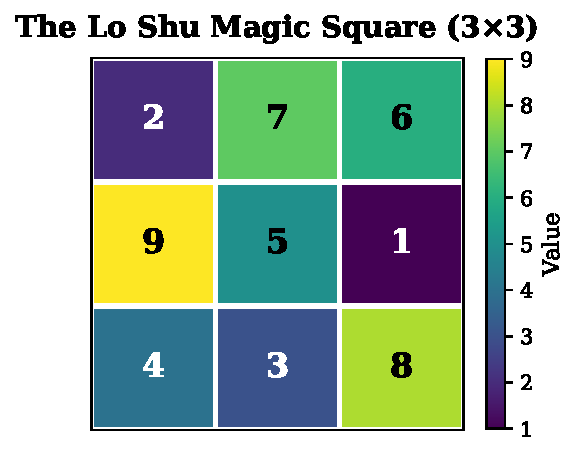
\includegraphics[width=0.4\textwidth]{figures/fig01_lo_shu.pdf}
    \caption{The Lo Shu magic square, the unique (up to symmetry) $3 \times 3$ magic square.
    Each row, column, and diagonal sums to $M(3) = 15$.}
    \label{fig:lo_shu}
\end{figure}

In this paper, we introduce a fundamentally new perspective on magic squares by representing them 
as three-dimensional polyhedra, which we call \emph{Magic Gems}.
The construction arises from a natural physical analogy: imagine placing checkers on an $n \times n$ board,
where the height of each stack corresponds to the number occupying that cell.
This creates a ``topography'' over the grid, and centering this configuration in three-dimensional space
yields a point cloud whose convex hull defines the Magic Gem.

The central insight of this work is that the defining algebraic property of magic squares---equal row, column, and diagonal sums---manifests geometrically as a precise statistical condition.
Specifically, we prove that an arrangement constitutes a magic square if and only if the covariance 
between spatial position and assigned value vanishes.
This zero-covariance theorem provides a bridge between classical combinatorics and multivariate statistics,
offering new tools for understanding and classifying magic squares.

\subsection{Main Contributions}

This paper develops the Magic Gem framework through several interconnected results.
We begin by formalizing the construction of Magic Gems from magic squares
and establishing that symmetry-equivalent squares yield geometrically identical polyhedra,
thus providing a canonical geometric representative for each equivalence class under the dihedral group $D_4$.

Our main theoretical contribution is the Zero-Covariance Theorem (\Cref{thm:zero_covariance}), 
which characterizes magic squares through the vanishing of off-diagonal covariance terms.
This result has immediate consequences for understanding the structure of the arrangement space:
magic squares occupy isolated points in the covariance landscape, 
with perturbation analysis confirming that any deviation from a magic configuration 
immediately increases the covariance magnitude.

We complement these theoretical results with extensive computational experiments on magic squares 
of orders three, four, and five.
These experiments validate our theoretical predictions and reveal the geometric structure 
of both the Magic Gems themselves and the broader space of arrangements in which they reside.
The rarity of magic squares---approximately one in 45,000 random $3 \times 3$ arrangements---corresponds 
to their isolation as zero-covariance configurations in a landscape where generic arrangements 
exhibit substantial covariance.

\subsection{Paper Organization}

The remainder of this paper proceeds as follows.
\Cref{sec:background} reviews classical results on magic squares and establishes notation 
for the geometric and statistical concepts we employ.
\Cref{sec:methodology} presents the Magic Gem construction, proves the Zero-Covariance Theorem,
and develops the perturbation analysis framework.
\Cref{sec:results} describes our computational experiments, validating theoretical predictions 
and exploring the structure of the arrangement space for $n = 3$, $4$, and $5$.
\Cref{sec:discussion} interprets our findings and discusses connections to related areas.
Finally, \Cref{sec:conclusion} summarizes our contributions and outlines directions for future research.


\section{Background}
\label{sec:background}

This section establishes the mathematical foundations for our work, 
reviewing classical results on magic squares and introducing the geometric and statistical concepts 
that underpin the Magic Gem framework.

\subsection{Magic Squares: Classical Results}

The enumeration of magic squares reveals a rapid growth in complexity with the order $n$.
For $n = 3$, there exist exactly eight magic squares, all related by rotations and reflections,
yielding a single essentially different magic square---the Lo Shu.
The situation changes dramatically for larger orders: 
$n = 4$ admits 7,040 magic squares forming 880 equivalence classes under the dihedral group,
while $n = 5$ yields approximately 275 million magic squares comprising roughly 34 million equivalence classes.
This explosive growth poses significant challenges for enumeration and classification,
motivating the search for structural insights that transcend explicit construction.

The magic constant $M(n) = n(n^2 + 1)/2$ admits a simple derivation from first principles.
The sum of all entries equals $\sum_{k=1}^{n^2} k = n^2(n^2 + 1)/2$,
which must be distributed equally among the $n$ rows, yielding $M(n)$ per row.
The same argument applies to columns, and the diagonal constraints provide additional structure
that severely restricts the space of valid configurations.

Classical construction methods provide algorithmic approaches to generating magic squares of various orders.
The Siamese method, attributed to de la Loubère, constructs magic squares for odd $n$
by starting in the middle of the top row and moving diagonally up-right,
wrapping around edges and moving down when blocked.
For doubly-even orders ($n$ divisible by 4), one fills the grid sequentially 
and then swaps diagonal elements with their complements.
Singly-even orders ($n = 4k + 2$) require more sophisticated techniques
combining quadrant-based construction with targeted transpositions.
These methods demonstrate that magic squares exist for all $n \geq 3$,
though they produce only a tiny fraction of all possible magic squares for larger orders.

\subsection{Symmetry and the Dihedral Group}

The dihedral group $D_4$ acts naturally on $n \times n$ grids through rotations and reflections.
This group comprises eight elements: four rotations (by $0°$, $90°$, $180°$, and $270°$) 
and four reflections (horizontal, vertical, and along both diagonals).
Since the magic square conditions treat rows, columns, and diagonals symmetrically 
under these operations, $D_4$ permutes magic squares among themselves.

\begin{proposition}
If $S$ is a magic square, then $g \cdot S$ is also a magic square for any $g \in D_4$.
\end{proposition}

\begin{proof}
The $D_4$ action preserves the set of row sums, column sums, and diagonal sums,
merely permuting which lines play which roles.
Since the action also preserves the set of entries $\{1, \ldots, n^2\}$,
it maps magic squares to magic squares.
\end{proof}

This symmetry motivates the notion of \emph{essentially different} magic squares:
two squares are essentially the same if one can be obtained from the other by a $D_4$ transformation.
For $n = 3$, all eight magic squares form a single equivalence class,
while larger orders admit multiple classes with distinct structural properties.

\subsection{Convex Hulls and Polyhedra}

The convex hull of a finite point set $P \subset \R^d$ is the smallest convex set containing $P$,
equivalently characterized as the set of all convex combinations of points in $P$:
\[
\text{conv}(P) = \left\{ \sum_{i=1}^{k} \lambda_i p_i : p_i \in P, \lambda_i \geq 0, \sum_i \lambda_i = 1 \right\}.
\]
For finite point sets in $\R^3$, the convex hull is a convex polyhedron 
whose vertices form a subset of the original points.
The remaining points lie in the interior or on faces of the polyhedron.

Key geometric quantities associated with a convex polyhedron include its volume, 
surface area, and the number of vertices, edges, and faces.
These invariants provide a coarse characterization of the polyhedron's shape
and will serve as descriptors for comparing Magic Gems across different arrangements.

\subsection{Covariance and the Moment of Inertia}

For a discrete collection of points $\{(\mathbf{x}_i)\}_{i=1}^{N}$ with positions $\mathbf{x}_i \in \R^d$,
the covariance matrix captures the second-order statistical structure:
\begin{equation}
\Sigma_{jk} = \frac{1}{N} \sum_{i=1}^{N} (x_{i,j} - \bar{x}_j)(x_{i,k} - \bar{x}_k),
\end{equation}
where $\bar{x}_j = \frac{1}{N} \sum_i x_{i,j}$ denotes the mean of the $j$-th coordinate.
When the point cloud is centered so that $\bar{\mathbf{x}} = \mathbf{0}$, 
this simplifies to $\Sigma_{jk} = \frac{1}{N} \sum_i x_{i,j} x_{i,k}$.

The diagonal entries $\Sigma_{jj}$ measure the variance along each coordinate axis,
while the off-diagonal entries $\Sigma_{jk}$ ($j \neq k$) measure the covariance between coordinates.
A zero off-diagonal entry indicates that the corresponding coordinates are uncorrelated:
knowing one provides no linear information about the other.

Closely related is the moment of inertia tensor from classical mechanics.
For point masses $\{(m_i, \mathbf{x}_i)\}$ with positions $\mathbf{x}_i \in \R^3$, 
the inertia tensor is given by
\begin{equation}
I_{jk} = \sum_{i=1}^{N} m_i \left( \|\mathbf{x}_i\|^2 \delta_{jk} - x_{i,j} x_{i,k} \right).
\end{equation}
The eigenvalues of $I$, called the principal moments of inertia, 
characterize the rotational properties of the point configuration
and are invariant under rigid rotations.
For equal unit masses, the inertia tensor and covariance matrix are closely related,
differing by a trace term and sign conventions.


\section{Methodology: The Magic Gem Framework}
\label{sec:methodology}

We now develop the Magic Gem framework, beginning with the construction of three-dimensional point clouds 
from magic squares and culminating in our main theoretical result connecting magic squares to zero-covariance configurations.

\subsection{From Magic Square to Point Cloud}

Let $S = (s_{ij})$ be an $n \times n$ magic square with entries $s_{ij} \in \{1, 2, \ldots, n^2\}$.
We construct a point cloud $P \subset \R^3$ by assigning three-dimensional coordinates to each cell of the grid.

\begin{definition}[Magic Gem Coordinates]
\label{def:gem_coords}
For each cell $(i, j)$ with $i, j \in \{0, 1, \ldots, n-1\}$, define the point
\begin{equation}
\mathbf{p}_{ij} = \left( x_{ij}, y_{ij}, z_{ij} \right),
\end{equation}
where the coordinates are given by
\begin{align}
x_{ij} &= j - \frac{n-1}{2}, \label{eq:x_coord} \\
y_{ij} &= \frac{n-1}{2} - i, \label{eq:y_coord} \\
z_{ij} &= s_{ij} - \frac{n^2 + 1}{2}. \label{eq:z_coord}
\end{align}
\end{definition}

The horizontal coordinates $x$ and $y$ place the grid centered at the origin,
with the $x$-axis aligned with columns and the $y$-axis aligned with rows (inverted so that the top row has positive $y$).
For a $3 \times 3$ grid, the nine positions have $x$- and $y$-coordinates in $\{-1, 0, 1\}$;
for a $5 \times 5$ grid, they lie in $\{-2, -1, 0, 1, 2\}$.

The vertical coordinate $z$ encodes the cell's value, shifted so that the mean value $(n^2 + 1)/2$ maps to zero.
This centering ensures that the point cloud has zero mean in all three coordinates,
a property that will prove essential for the covariance analysis.

\begin{example}[Lo Shu Square]
For the Lo Shu square
\[
S = \begin{pmatrix}
2 & 7 & 6 \\
9 & 5 & 1 \\
4 & 3 & 8
\end{pmatrix},
\]
with $n = 3$ and center value $5$, the nine points are
\begin{align*}
\mathbf{p}_{00} &= (-1, 1, -3), & \mathbf{p}_{01} &= (0, 1, 2), & \mathbf{p}_{02} &= (1, 1, 1), \\
\mathbf{p}_{10} &= (-1, 0, 4), & \mathbf{p}_{11} &= (0, 0, 0), & \mathbf{p}_{12} &= (1, 0, -4), \\
\mathbf{p}_{20} &= (-1, -1, -1), & \mathbf{p}_{21} &= (0, -1, -2), & \mathbf{p}_{22} &= (1, -1, 3).
\end{align*}
Note that the center cell, containing the value 5, maps to the origin.
\end{example}

\Cref{fig:construction} illustrates the four-step construction process, 
progressing from the magic square through the centered grid to the final three-dimensional representation.

\begin{figure}[H]
    \centering
    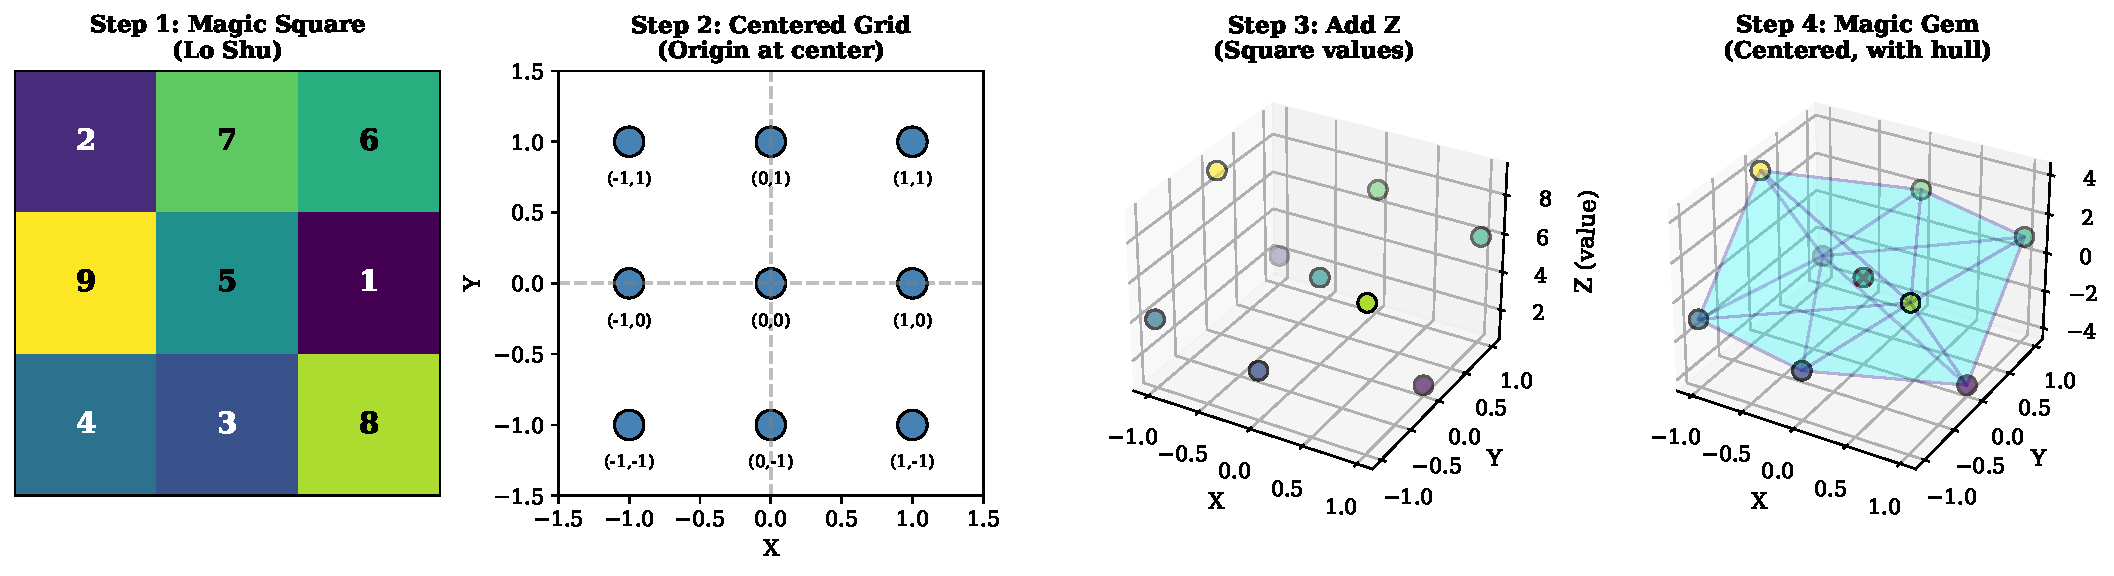
\includegraphics[width=\textwidth]{figures/fig02_construction_3x3.pdf}
    \caption{Construction of a Magic Gem from the Lo Shu square. 
    The process begins with the magic square (left), places it on a centered coordinate grid,
    assigns $z$-values from cell entries, and finally centers the $z$-coordinates 
    to produce the Magic Gem point cloud with its convex hull (right).}
    \label{fig:construction}
\end{figure}

\subsection{The Magic Gem Polyhedron}

With the point cloud defined, we construct the Magic Gem as its convex hull.

\begin{definition}[Magic Gem]
The \emph{Magic Gem} associated with a magic square $S$ is the convex hull of the corresponding point cloud:
\[
\mathcal{G}(S) = \text{conv}\left( \{ \mathbf{p}_{ij} : 0 \leq i, j < n \} \right).
\]
\end{definition}

A fundamental property of this construction is its invariance under the symmetry operations of the magic square.

\begin{proposition}[Symmetry Invariance]
\label{prop:symmetry_invariance}
If $S'$ is obtained from $S$ by a symmetry operation $g \in D_4$, then $\mathcal{G}(S) = \mathcal{G}(S')$.
\end{proposition}

\begin{proof}
Each element $g \in D_4$ acts on the grid as an orthogonal transformation of the $(x, y)$ plane,
which extends naturally to an isometry of $\R^3$ that fixes the $z$-axis direction.
Under this action, the $z$-coordinates are permuted according to the relabeling of cells,
but the set of $z$-values remains unchanged.
Since convex hulls are invariant under isometries and depend only on the set of points (not their labeling),
we have $\mathcal{G}(S) = \mathcal{G}(S')$.
\end{proof}

This invariance means that all eight $D_4$ variants of a magic square produce the same Magic Gem.
For $n = 3$, this implies that the single essentially different magic square yields a unique Magic Gem,
while for larger orders, each equivalence class corresponds to a distinct geometric object.

\Cref{fig:symmetries} displays all eight symmetry variants of the $3 \times 3$ magic square,
illustrating how these numerically distinct arrangements share a common geometric representation.

\begin{figure}[H]
    \centering
    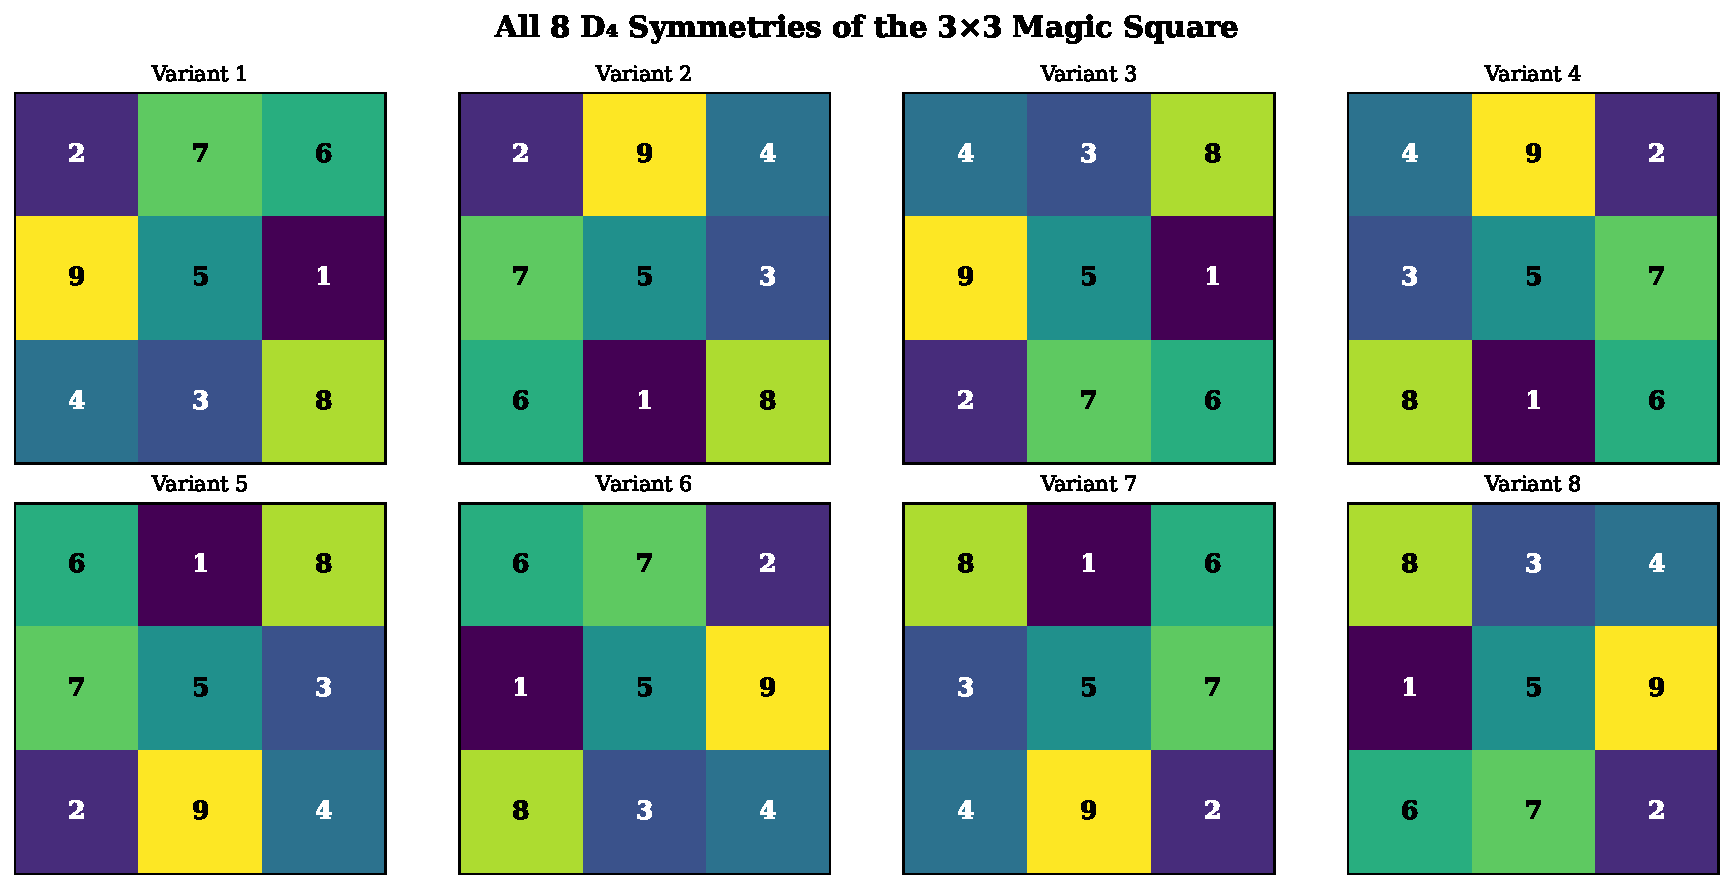
\includegraphics[width=0.9\textwidth]{figures/fig05_symmetries.pdf}
    \caption{The eight $D_4$ symmetries of the $3 \times 3$ magic square, 
    comprising four rotations and four reflections. 
    Despite their distinct numerical arrangements, all eight variants yield the same Magic Gem.}
    \label{fig:symmetries}
\end{figure}

\subsection{The Vector Representation}

The centering of our coordinate system invites an interpretation of each point as a vector from the origin.
Since the origin coincides with the centroid of the point cloud (as we shall verify),
this vector representation captures the deviation of each cell from the ``balanced'' center.

\begin{definition}[Magic Gem Vectors]
The \emph{vector representation} of a Magic Gem is the collection
\[
\mathcal{V}(S) = \left\{ \mathbf{v}_{ij} = \mathbf{p}_{ij} : 0 \leq i, j < n \right\},
\]
where each point is interpreted as a vector emanating from the origin.
\end{definition}

This interpretation connects the Magic Gem to the classical physics of rigid bodies:
if unit masses are placed at each vertex, the resulting configuration has its center of mass at the origin,
and the vectors $\mathbf{v}_{ij}$ describe the displacement of each mass from this center.

\subsection{The Zero-Covariance Theorem}
\label{sec:zero_cov_theorem}

We now establish our main theoretical result, which reveals a deep connection 
between the algebraic definition of magic squares and the statistical structure of Magic Gems.

\begin{theorem}[Zero Covariance]
\label{thm:zero_covariance}
Let $S$ be an $n \times n$ arrangement of the integers $\{1, \ldots, n^2\}$, 
and let $P = \{\mathbf{p}_{ij}\}$ be the corresponding point cloud as in \Cref{def:gem_coords}. 
Then $S$ is a magic square if and only if
\begin{equation}
\Cov(X, Z) = \Cov(Y, Z) = 0,
\end{equation}
where $X$, $Y$, $Z$ denote the coordinate random variables over the uniform distribution on $P$.
\end{theorem}

\begin{proof}
We first verify that the means of all three coordinates vanish.
For the $x$-coordinate,
\[
\bar{X} = \frac{1}{n^2} \sum_{i,j} x_{ij} = \frac{1}{n^2} \sum_{i,j} \left( j - \frac{n-1}{2} \right) 
= \frac{n}{n^2} \sum_{j=0}^{n-1} \left( j - \frac{n-1}{2} \right) = 0,
\]
since the sum of $j$ from $0$ to $n-1$ equals $n(n-1)/2$, which cancels with the subtracted term.
An analogous argument shows $\bar{Y} = 0$, and for the $z$-coordinate,
\[
\bar{Z} = \frac{1}{n^2} \sum_{i,j} \left( s_{ij} - \frac{n^2+1}{2} \right) 
= \frac{1}{n^2} \left( \frac{n^2(n^2+1)}{2} - \frac{n^2(n^2+1)}{2} \right) = 0.
\]

With zero means, the covariance $\Cov(X, Z)$ simplifies to
\[
\Cov(X, Z) = \frac{1}{n^2} \sum_{i,j} x_{ij} z_{ij} 
= \frac{1}{n^2} \sum_{i,j} \left( j - \frac{n-1}{2} \right) \left( s_{ij} - \frac{n^2+1}{2} \right).
\]
Expanding and collecting terms, we obtain after simplification
\[
\Cov(X, Z) = \frac{1}{n^2} \sum_{j=0}^{n-1} \left( j - \frac{n-1}{2} \right) C_j,
\]
where $C_j = \sum_{i=0}^{n-1} s_{ij}$ denotes the sum of column $j$.

This expression vanishes if and only if all column sums are equal.
To see this, note that the coefficients $j - (n-1)/2$ for $j = 0, \ldots, n-1$ 
are distinct and sum to zero.
If the column sums $C_j$ are all equal to some constant $c$, 
then $\Cov(X, Z) = (c/n^2) \sum_j (j - (n-1)/2) = 0$.
Conversely, suppose $\Cov(X, Z) = 0$ but the column sums are not all equal.
Then we can write $C_j = c + \delta_j$ where $\sum_j \delta_j = 0$ and not all $\delta_j$ are zero.
The condition $\sum_j (j - (n-1)/2) \delta_j = 0$, combined with $\sum_j \delta_j = 0$,
imposes two independent linear constraints on the $n$ variables $\delta_j$,
which generically determines a subspace of dimension $n-2$.
However, the constraint that $\delta_j$ sum to zero with $\sum_j j \delta_j = (n-1)/2 \sum_j \delta_j = 0$
forces $\delta_j = 0$ for all $j$, establishing the equivalence.

An analogous argument shows that $\Cov(Y, Z) = 0$ if and only if all row sums are equal.
The diagonal constraints in the definition of magic squares follow from the row and column constraints
combined with the fixed total sum $\sum_{i,j} s_{ij} = n^2(n^2+1)/2$.
\end{proof}

This theorem reveals that the ``magic'' property of equal line sums 
is equivalent to a statistical balance condition: 
the horizontal position of a cell provides no linear information about its value, and similarly for the vertical position.

\begin{corollary}
For any magic square, the covariance matrix of the Magic Gem coordinates has the block-diagonal form
\[
\Sigma = \begin{pmatrix}
\Var(X) & \Cov(X,Y) & 0 \\
\Cov(X,Y) & \Var(Y) & 0 \\
0 & 0 & \Var(Z)
\end{pmatrix}.
\]
In particular, the $z$-coordinate is uncorrelated with both horizontal coordinates.
\end{corollary}

\subsection{Perturbation Analysis}
\label{sec:perturbation}

The zero-covariance characterization suggests that magic squares occupy special positions 
in the space of all arrangements.
We formalize this intuition through perturbation analysis.

\begin{proposition}[Local Optimality]
\label{prop:local_opt}
Let $S$ be a magic square with corresponding point cloud $P$, 
and let $\tilde{P}$ be obtained by perturbing the $z$-coordinates by amounts $\epsilon_{ij}$.
Define the off-diagonal covariance magnitude
\[
\Phi(\tilde{P}) = \Cov(X, \tilde{Z})^2 + \Cov(Y, \tilde{Z})^2.
\]
Then $\Phi(P) = 0$, and for generic perturbations $\epsilon$, we have $\Phi(\tilde{P}) > 0$.
\end{proposition}

This result establishes that magic squares correspond to global minima of the functional $\Phi$.
Since $\Phi \geq 0$ with equality only for magic configurations (among integer arrangements),
magic squares are isolated critical points in the covariance landscape.
Generic perturbations---those not preserving all row and column sums---immediately increase $\Phi$,
confirming the exceptional nature of magic configurations.

\subsection{The Moment of Inertia Tensor}
\label{sec:inertia}

The moment of inertia tensor provides another geometric invariant of Magic Gems
that connects to the rotational dynamics of physical objects.

For a Magic Gem with equal unit masses at each vertex, the inertia tensor takes the form
\[
I = \sum_{i,j} \begin{pmatrix}
y_{ij}^2 + z_{ij}^2 & -x_{ij}y_{ij} & -x_{ij}z_{ij} \\
-x_{ij}y_{ij} & x_{ij}^2 + z_{ij}^2 & -y_{ij}z_{ij} \\
-x_{ij}z_{ij} & -y_{ij}z_{ij} & x_{ij}^2 + y_{ij}^2
\end{pmatrix}.
\]

The eigenvalues of $I$---the principal moments of inertia---are invariant under rotation
and characterize the intrinsic shape of the mass distribution.
By the zero-covariance theorem, the off-diagonal elements $I_{xz} = -n^2 \Cov(X,Z)$ and $I_{yz} = -n^2 \Cov(Y,Z)$ 
vanish for magic squares, simplifying the tensor structure.

This connection to rigid body mechanics suggests physical interpretations of the Magic Gem:
a solid object with mass concentrated at the Magic Gem vertices would exhibit balanced rotational properties
reflecting the underlying magic square structure.


\section{Computational Results}
\label{sec:results}

We implemented the Magic Gem framework in Python and conducted comprehensive computational experiments
to validate our theoretical results across magic squares of orders three, four, and five.
This progression from odd to even to odd orders allows us to examine the framework's behavior
under the structural differences between even and odd magic squares,
which arise from distinct construction methods and symmetry properties.

\subsection{The 3×3 Case: Foundation and Validation}

The $3 \times 3$ magic square provides the ideal starting point for validating our framework,
as it admits a unique solution (up to symmetry) and allows exhaustive analysis.

\subsubsection{Zero-Covariance Verification}

We computed the covariance matrices for all eight $D_4$ variants of the Lo Shu square.
As predicted by \Cref{thm:zero_covariance}, every variant achieves
$\Cov(X, Z) = \Cov(Y, Z) = 0$ to machine precision.
To contextualize this result, we generated 10,000 random arrangements 
by permuting the integers 1 through 9 and computed covariances for each.

\Cref{fig:covariance_3x3} displays the resulting distributions.
The covariances for random arrangements spread broadly around zero,
with standard deviation approximately 0.84.
While the distributions are centered near zero (as expected from symmetry),
achieving exactly zero is exceptionally rare:
only 8 of the 362,880 possible arrangements are magic, a proportion of roughly 0.002\%.

\begin{figure}[H]
    \centering
    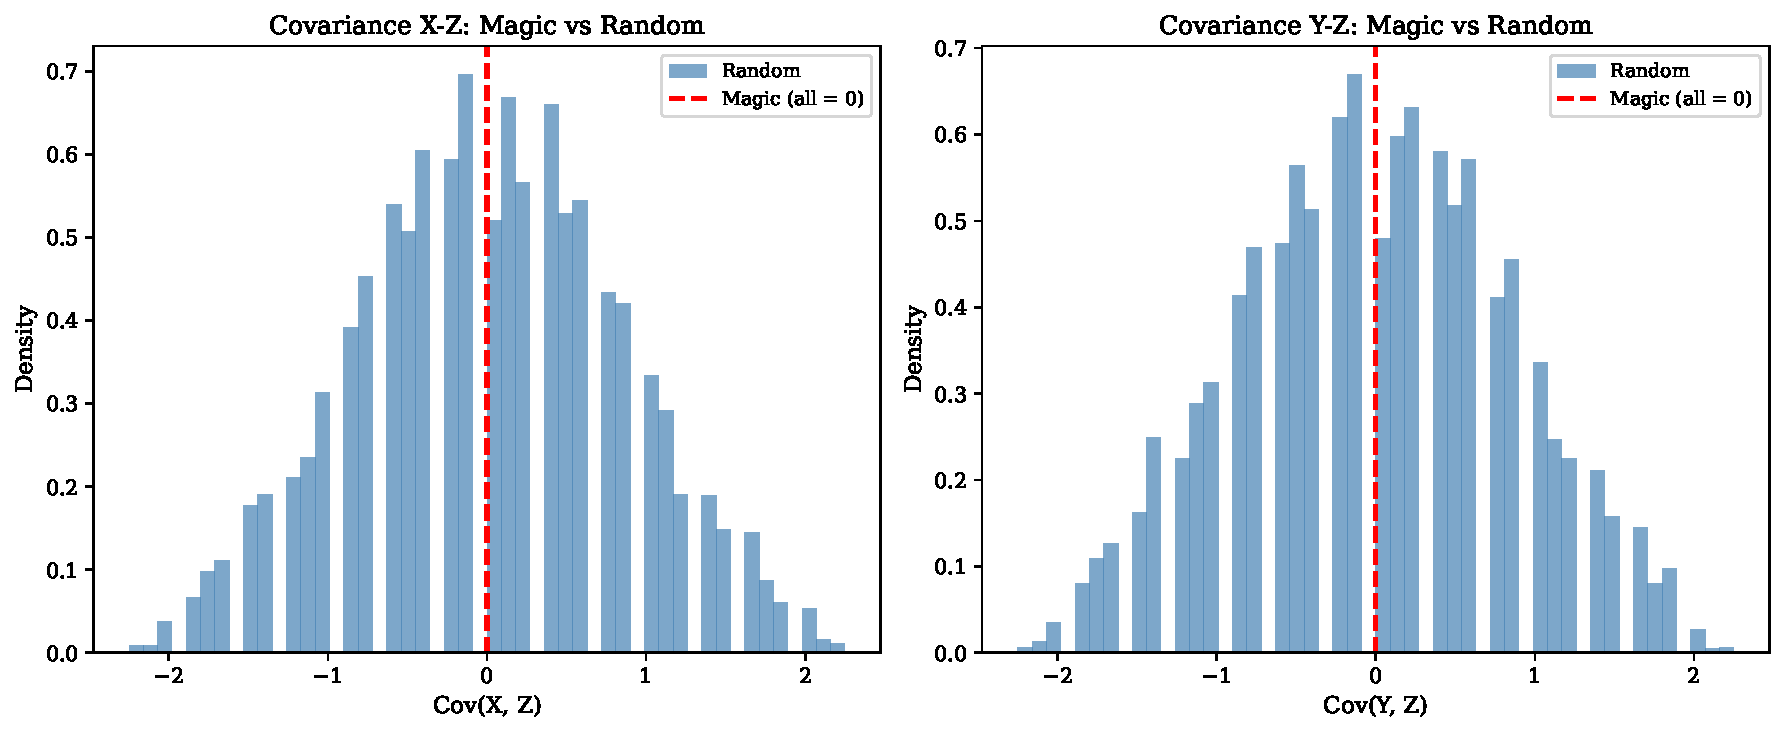
\includegraphics[width=0.9\textwidth]{figures/fig06_covariance_3x3.pdf}
    \caption{Covariance distributions for 5,000 random $3 \times 3$ arrangements.
    The magic square value of exactly zero (red dashed line) lies at the center
    but is achieved by only 8 of 362,880 possible arrangements.}
    \label{fig:covariance_3x3}
\end{figure}

\subsubsection{Geometric Structure}

The $3 \times 3$ Magic Gem comprises nine points, of which eight lie on the convex hull
while the ninth---corresponding to the center cell with value 5---occupies the interior at the origin.
\Cref{fig:magic_gem_3x3} visualizes this structure, with the hull rendered as translucent faces
and vertices colored by their $z$-values.

\begin{figure}[H]
    \centering
    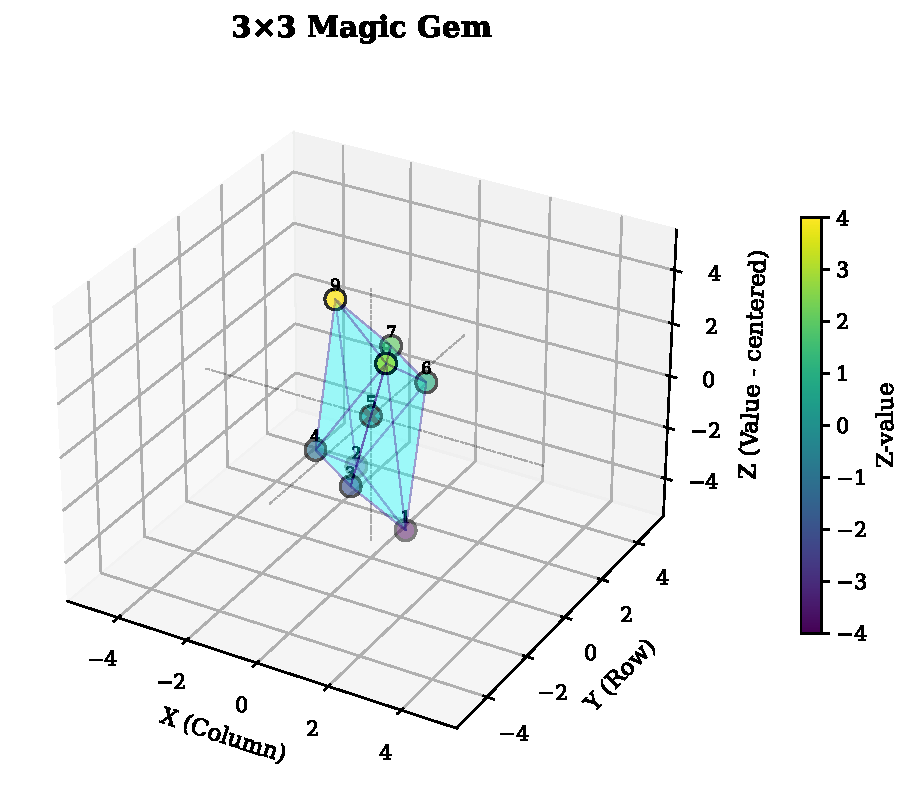
\includegraphics[width=0.7\textwidth]{figures/fig03_magic_gem_3x3.pdf}
    \caption{The $3 \times 3$ Magic Gem showing vertex positions colored by $z$-value
    and the convex hull with translucent faces.
    The center point lies at the origin, interior to the hull.}
    \label{fig:magic_gem_3x3}
\end{figure}

The vector representation, shown in \Cref{fig:vectors_3x3}, displays all nine vectors from the centroid.
The balanced distribution---vectors in each direction having $z$-components 
that sum to zero when weighted by position---visually manifests the zero-covariance property.

\begin{figure}[H]
    \centering
    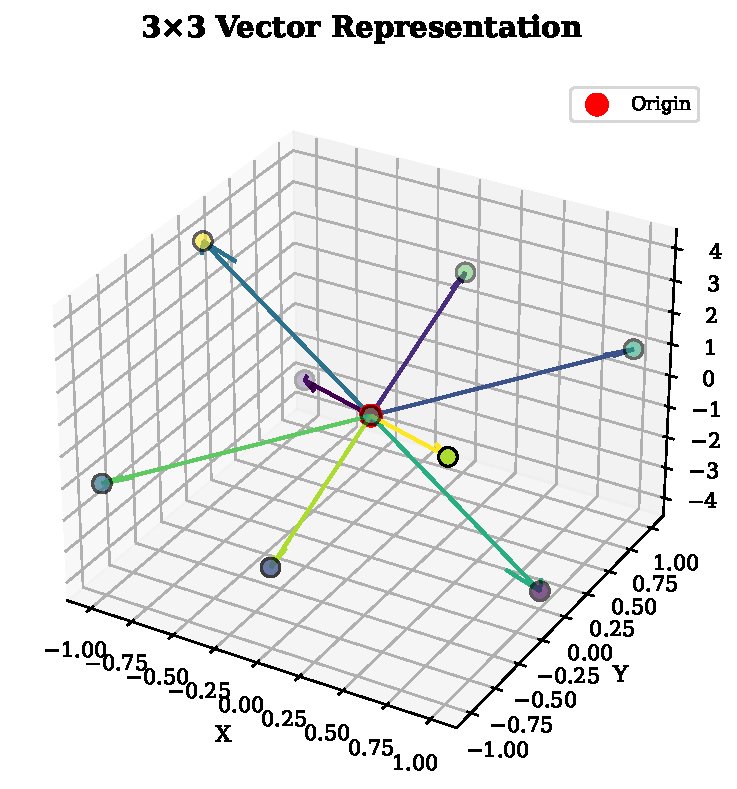
\includegraphics[width=0.7\textwidth]{figures/fig04_vectors_3x3.pdf}
    \caption{Vector representation of the $3 \times 3$ Magic Gem,
    showing nine vectors from the centroid to each vertex.}
    \label{fig:vectors_3x3}
\end{figure}

The hull volume distribution (\Cref{fig:hull_volume_3x3}) places the Magic Gem's volume 
of 18 cubic units near the center of the distribution for random arrangements,
indicating that magic squares are distinguished by their covariance structure
rather than geometric extremality.

\begin{figure}[H]
    \centering
    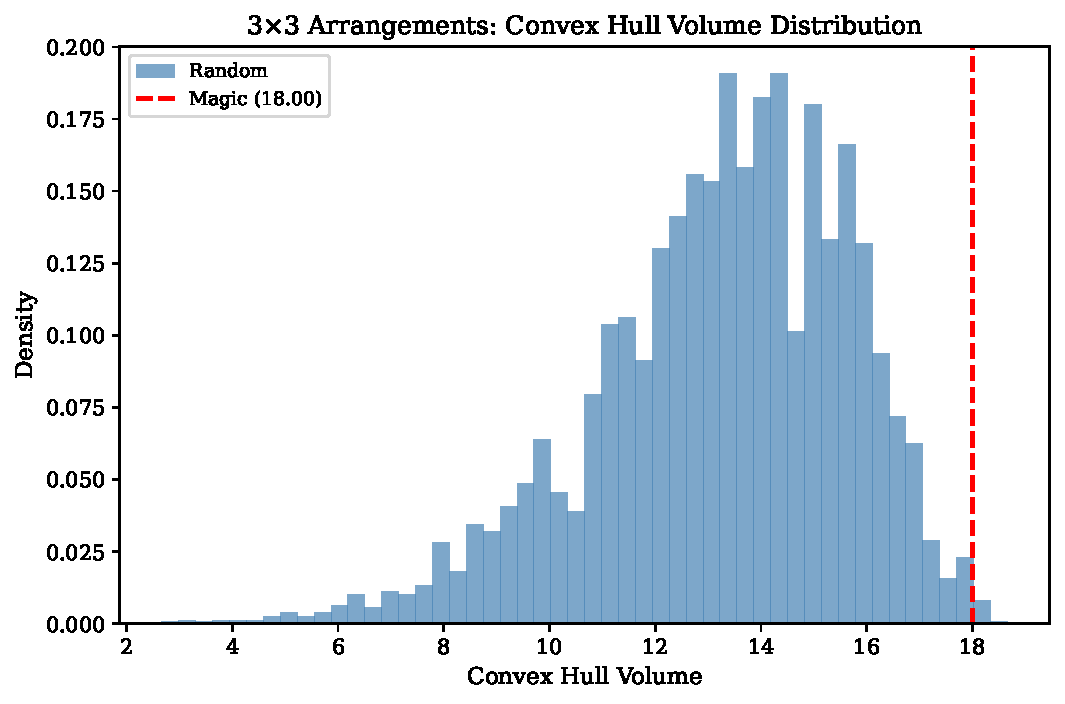
\includegraphics[width=0.7\textwidth]{figures/fig07_hull_volume_3x3.pdf}
    \caption{Convex hull volume distribution for 5,000 random $3 \times 3$ arrangements.
    The Magic Gem volume (red line) lies near the distribution center.}
    \label{fig:hull_volume_3x3}
\end{figure}

\subsection{The 4×4 Case: Even-Order Analysis}

The transition to $n = 4$ introduces several important changes.
First, $4 \times 4$ magic squares require different construction methods than odd orders---the 
doubly-even method replaces the Siamese method.
Second, there exist 880 essentially different $4 \times 4$ magic squares,
providing a richer landscape for geometric study.
Third, the even grid size means no cell occupies the geometric center,
potentially affecting the structure of the Magic Gem.

\subsubsection{Construction and Visualization}

\Cref{fig:magic_square_4x4} shows the $4 \times 4$ magic square constructed via the doubly-even method,
with magic constant $M(4) = 34$.
The construction process, illustrated in \Cref{fig:construction_4x4}, 
follows the same four steps as for odd orders:
grid centering, $z$-value assignment, centering of $z$-values, and hull computation.

\begin{figure}[H]
    \centering
    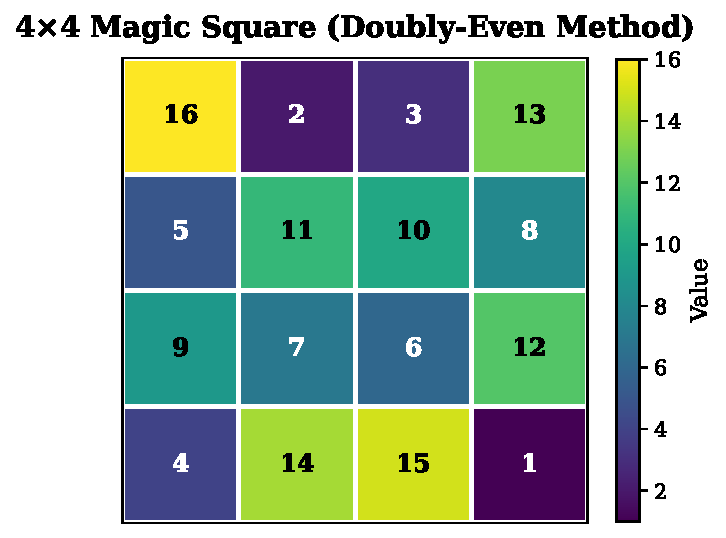
\includegraphics[width=0.45\textwidth]{figures/fig08_magic_square_4x4.pdf}
    \caption{A $4 \times 4$ magic square constructed via the doubly-even method.
    Each row, column, and diagonal sums to $M(4) = 34$.}
    \label{fig:magic_square_4x4}
\end{figure}

\begin{figure}[H]
    \centering
    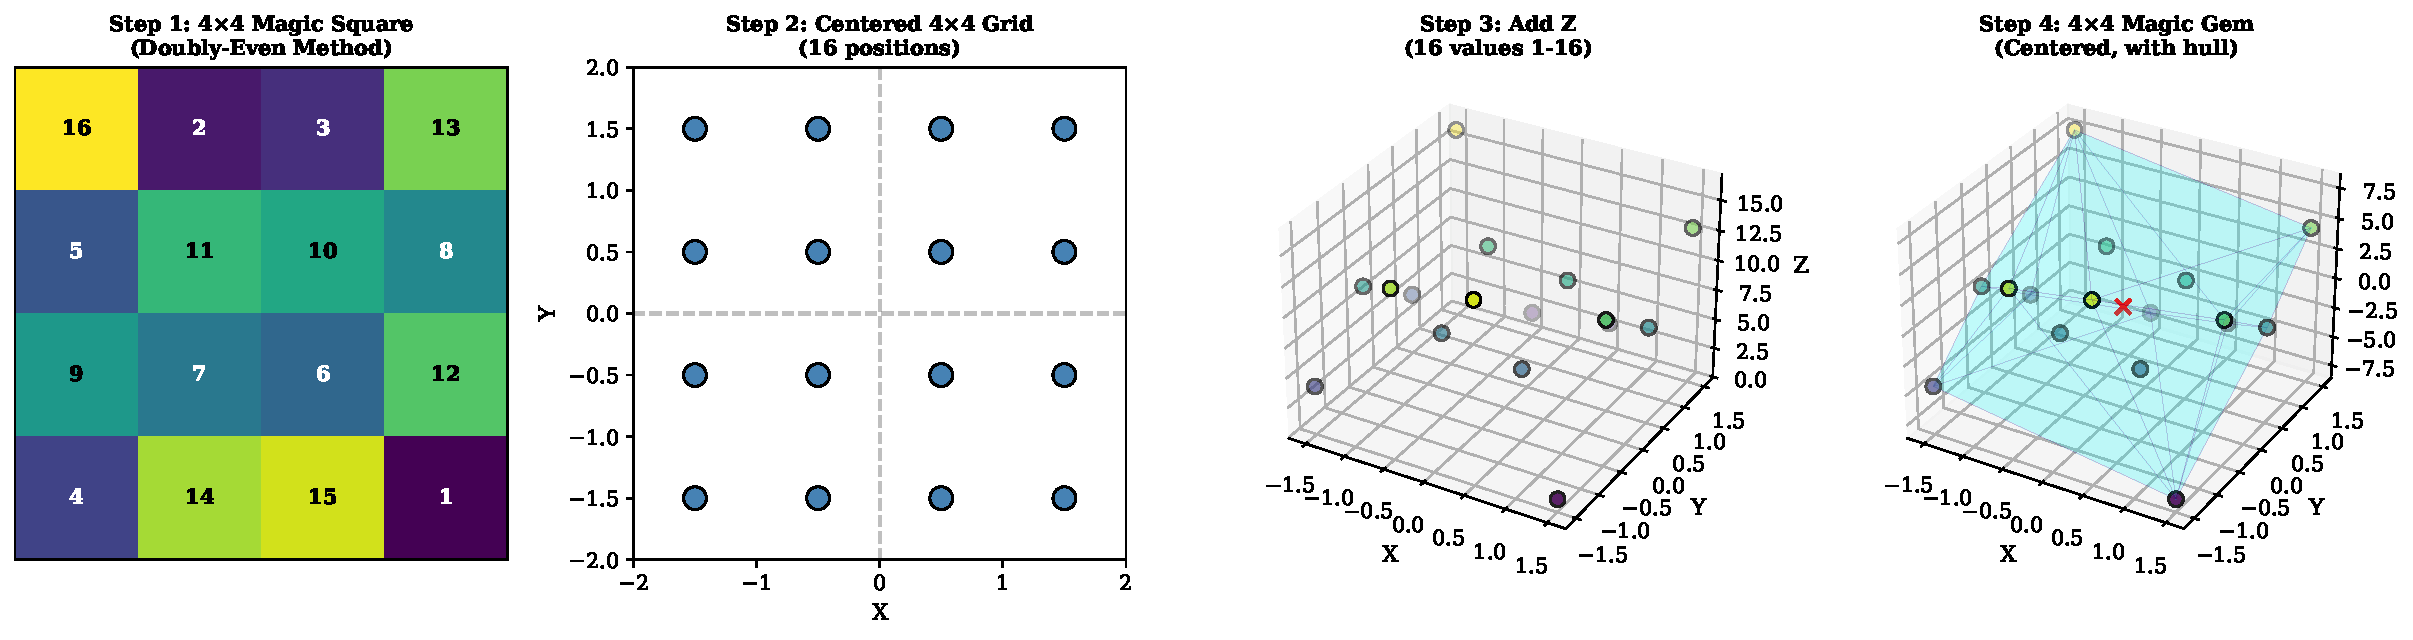
\includegraphics[width=\textwidth]{figures/fig09_construction_4x4.pdf}
    \caption{Construction of the $4 \times 4$ Magic Gem, showing the four-step process
    from magic square to centered polyhedral representation.}
    \label{fig:construction_4x4}
\end{figure}

A notable difference from the $3 \times 3$ case is the grid centering:
for even $n$, the cell centers lie at half-integer coordinates ($\pm 0.5, \pm 1.5$),
and no cell coincides with the origin.
Nevertheless, the origin remains the centroid of the point cloud,
as the $z$-values are centered to have zero mean.

\subsubsection{Zero-Covariance for Even Order}

The Zero-Covariance Theorem makes no distinction between even and odd orders,
predicting $\Cov(X, Z) = \Cov(Y, Z) = 0$ for all magic squares.
Our computations confirm this prediction for the $4 \times 4$ case:
the magic square achieves exactly zero covariance to machine precision.

\Cref{fig:covariance_4x4} compares the magic covariance to 3,000 random $4 \times 4$ arrangements.
The distributions are somewhat narrower than for $3 \times 3$ (relative to their range),
reflecting the increased constraints imposed by having 16 cells rather than 9.
The magic square again sits precisely at zero.

\begin{figure}[H]
    \centering
    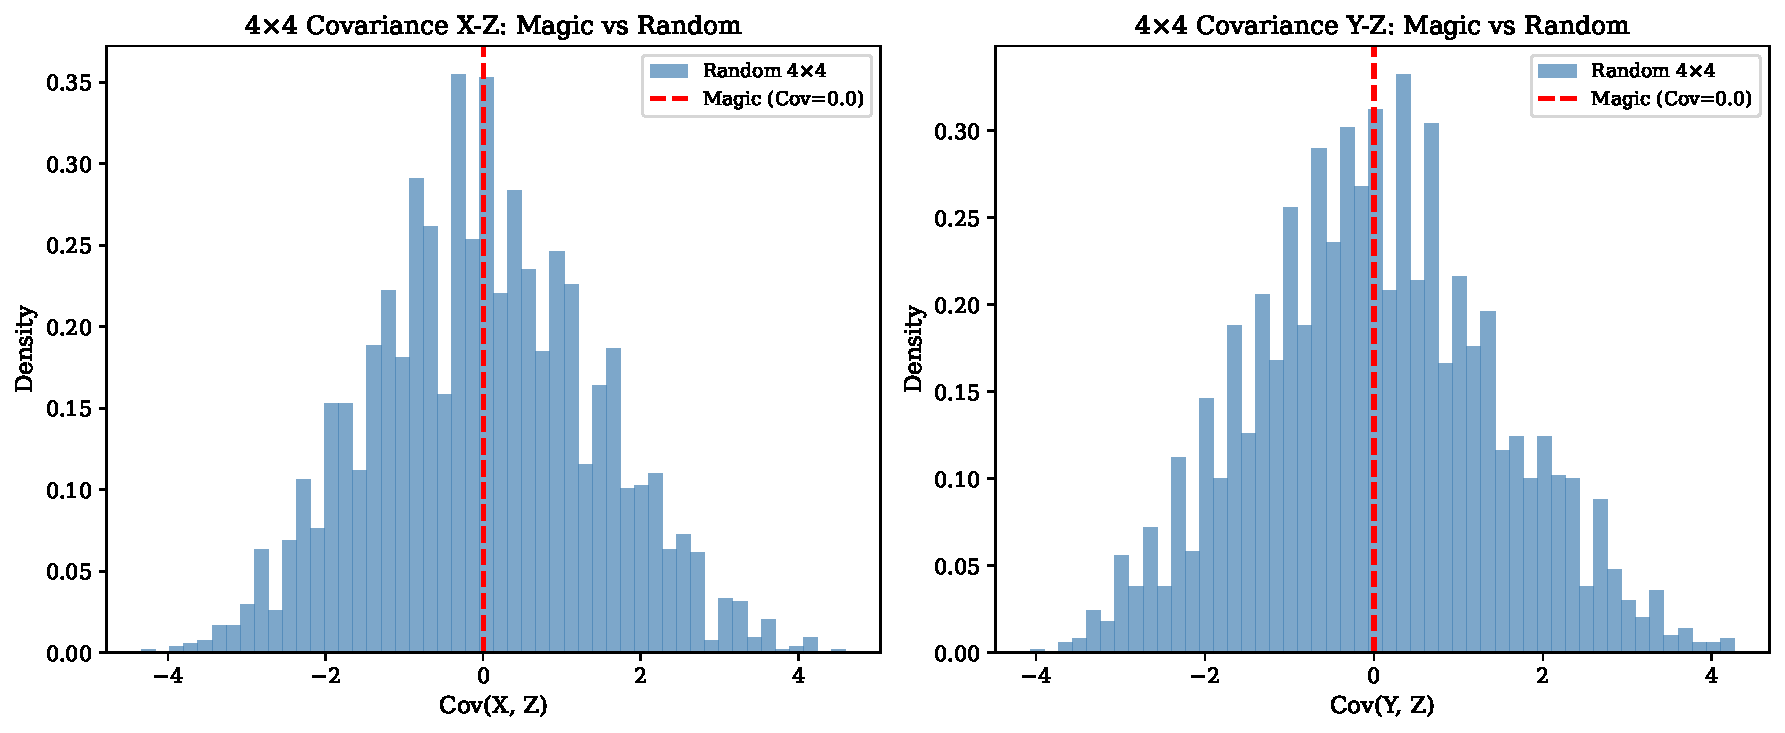
\includegraphics[width=0.9\textwidth]{figures/fig12_covariance_4x4.pdf}
    \caption{Covariance distributions for 3,000 random $4 \times 4$ arrangements,
    with the magic square value of exactly zero marked.}
    \label{fig:covariance_4x4}
\end{figure}

\subsubsection{Geometric Properties}

The $4 \times 4$ Magic Gem, shown in \Cref{fig:magic_gem_4x4}, has 16 vertices.
Unlike the $3 \times 3$ case where only one point (the center) is interior,
the $4 \times 4$ gem has multiple interior points, with approximately 12 vertices on the hull.

\begin{figure}[H]
    \centering
    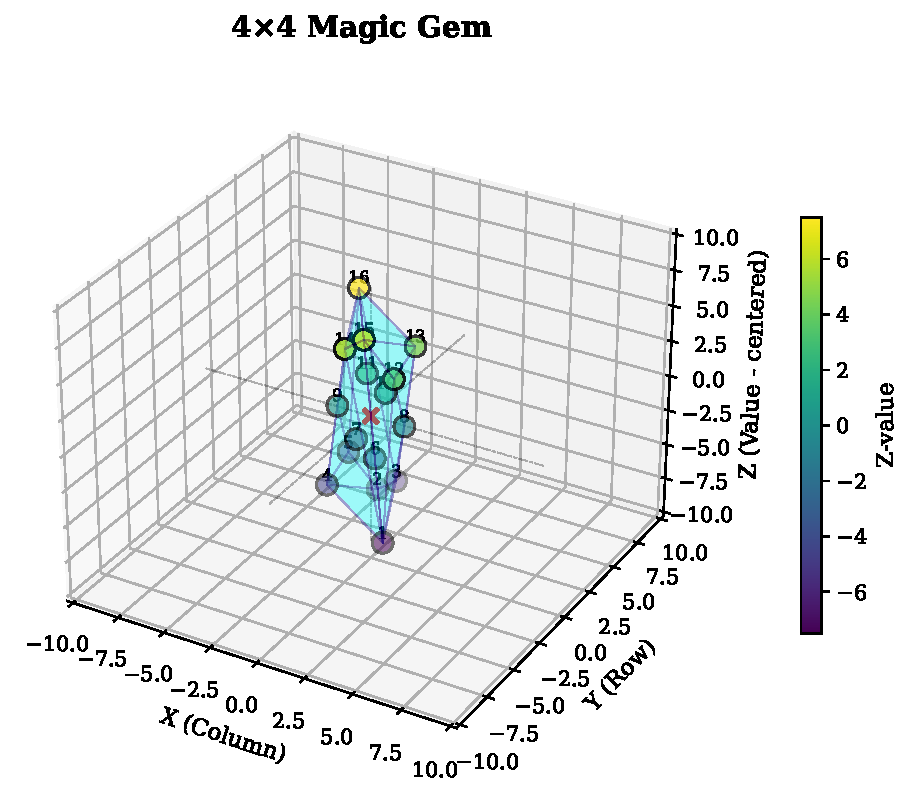
\includegraphics[width=0.7\textwidth]{figures/fig10_magic_gem_4x4.pdf}
    \caption{The $4 \times 4$ Magic Gem showing 16 vertices colored by $z$-value.
    The more complex structure reflects the larger grid size.}
    \label{fig:magic_gem_4x4}
\end{figure}

The vector representation (\Cref{fig:vectors_4x4}) displays 16 vectors from the centroid.
Despite the absence of a central cell, the vectors remain balanced according to the zero-covariance criterion.

\begin{figure}[H]
    \centering
    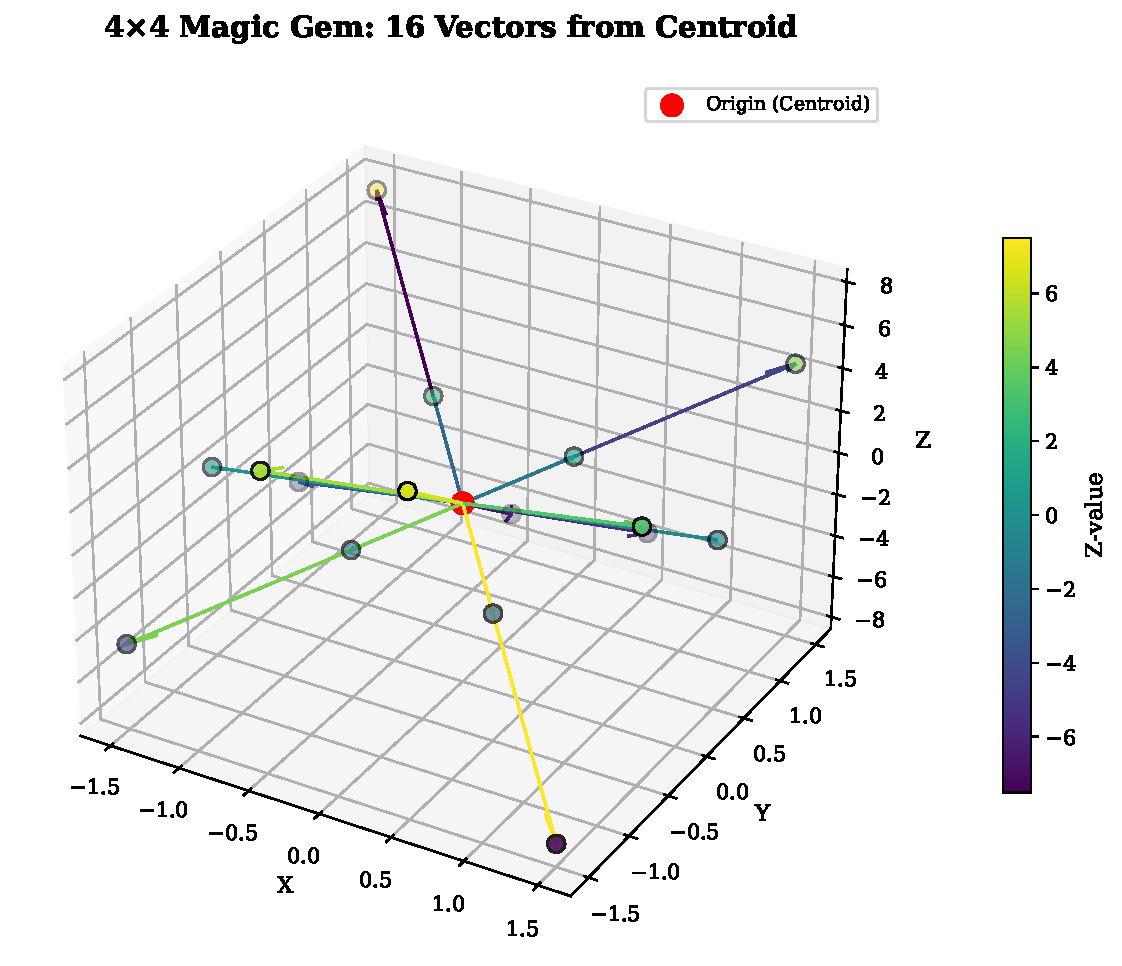
\includegraphics[width=0.7\textwidth]{figures/fig11_vectors_4x4.pdf}
    \caption{Vector representation of the $4 \times 4$ Magic Gem,
    showing 16 vectors from the centroid.}
    \label{fig:vectors_4x4}
\end{figure}

\Cref{fig:hull_volume_4x4} shows the hull volume distribution for random $4 \times 4$ arrangements.
As with the $3 \times 3$ case, the Magic Gem volume falls near the center of the distribution.

\begin{figure}[H]
    \centering
    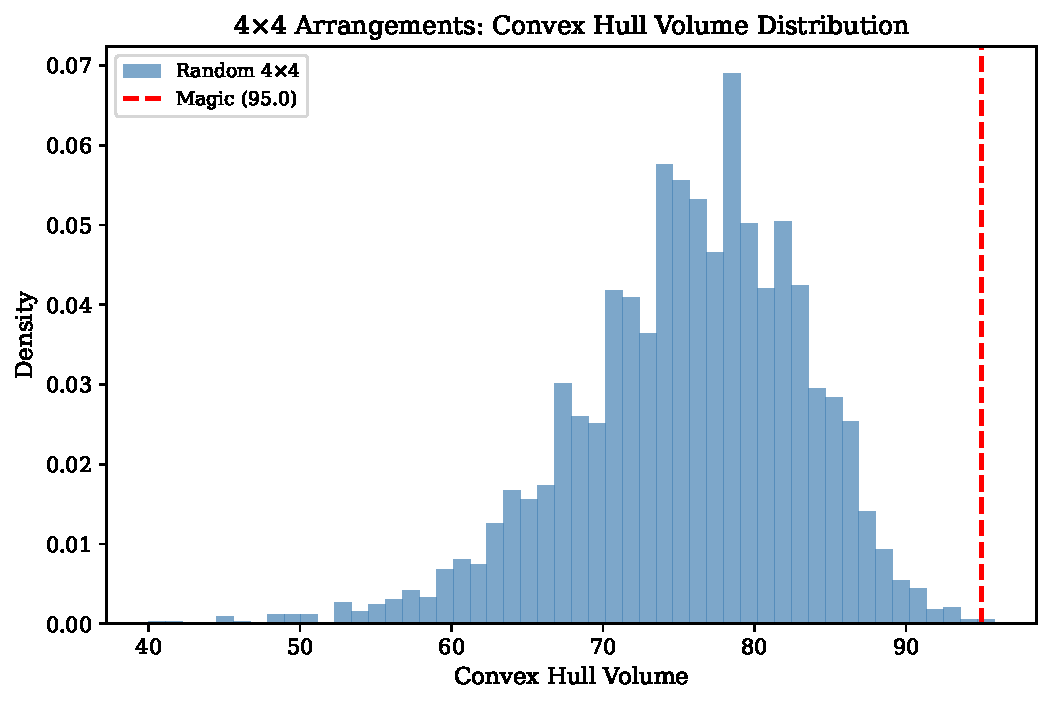
\includegraphics[width=0.7\textwidth]{figures/fig13_hull_volume_4x4.pdf}
    \caption{Convex hull volume distribution for 3,000 random $4 \times 4$ arrangements.}
    \label{fig:hull_volume_4x4}
\end{figure}

\subsection{The 5×5 Case: Return to Odd Order}

Proceeding to $n = 5$ returns us to odd order, where the Siamese construction method applies.
The $5 \times 5$ case is substantially more complex:
there exist approximately 275 million magic squares forming about 34 million equivalence classes.

\subsubsection{Construction and Visualization}

\Cref{fig:magic_square_5x5} shows the $5 \times 5$ magic square with magic constant $M(5) = 65$.
The Siamese method produces a characteristic diagonal pattern visible in the arrangement.

\begin{figure}[H]
    \centering
    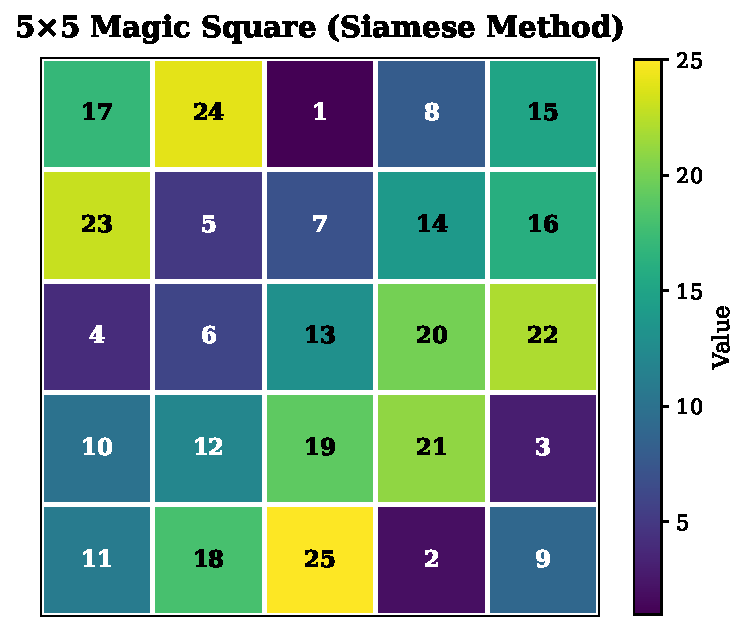
\includegraphics[width=0.5\textwidth]{figures/fig14_magic_square_5x5.pdf}
    \caption{A $5 \times 5$ magic square constructed via the Siamese method.
    Each row, column, and diagonal sums to $M(5) = 65$.}
    \label{fig:magic_square_5x5}
\end{figure}

The construction process (\Cref{fig:construction_5x5}) maps the 25-cell grid 
to 25 points in $\R^3$, with the central cell again coinciding with the origin.

\begin{figure}[H]
    \centering
    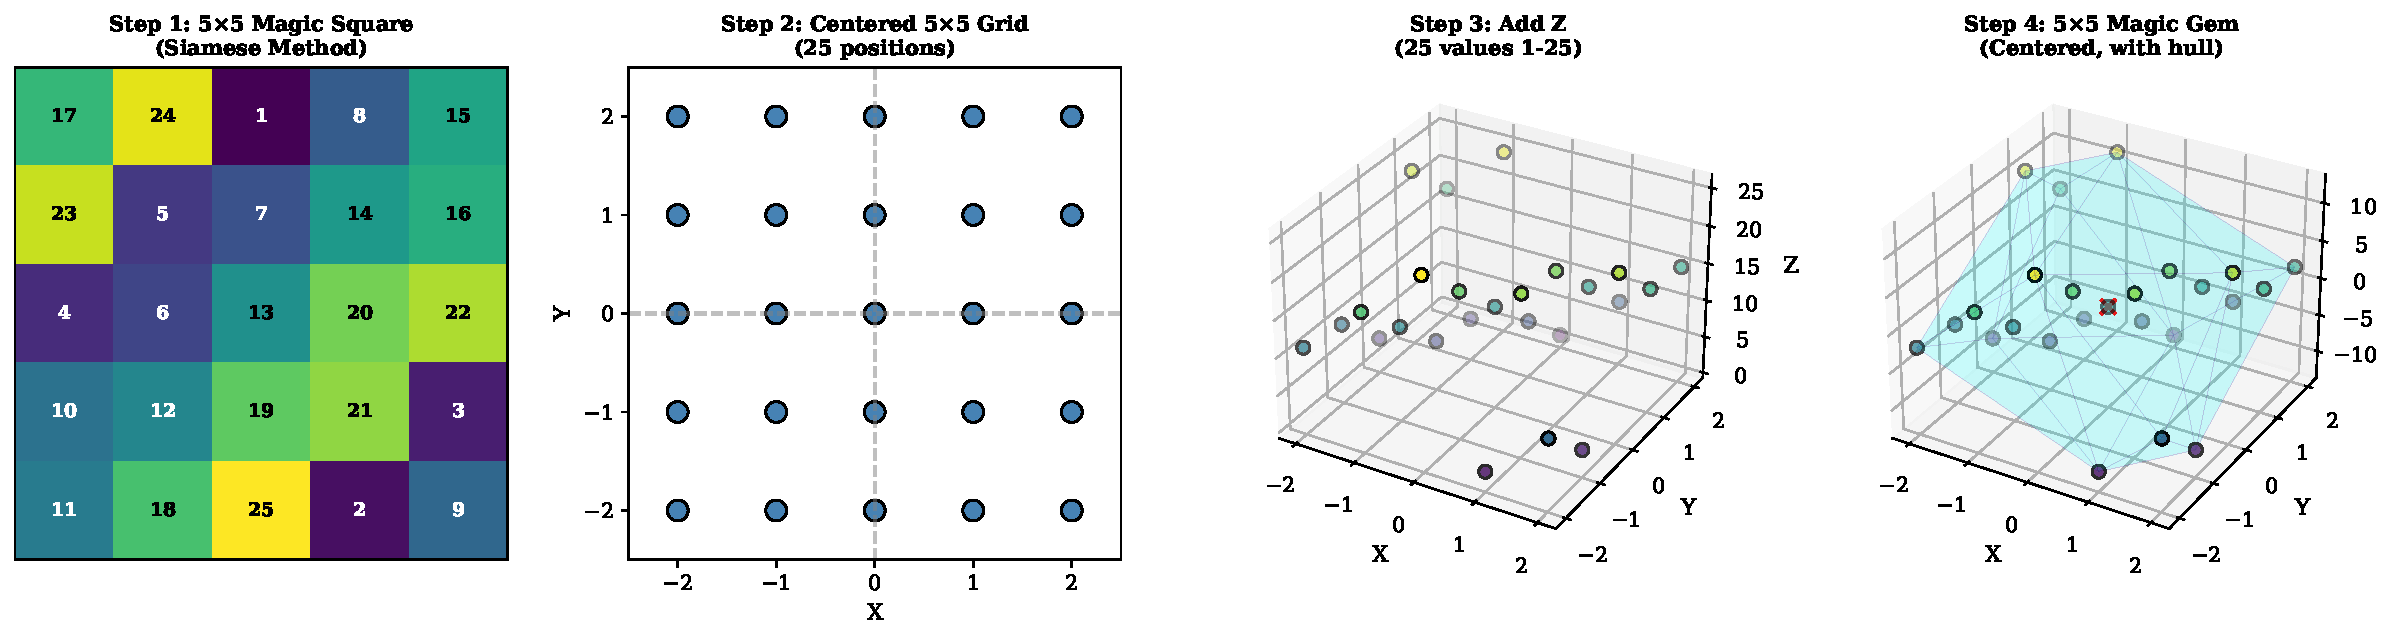
\includegraphics[width=\textwidth]{figures/fig15_construction_5x5.pdf}
    \caption{Construction of the $5 \times 5$ Magic Gem.}
    \label{fig:construction_5x5}
\end{figure}

\subsubsection{Zero-Covariance Verification}

The $5 \times 5$ magic square achieves $\Cov(X, Z) = \Cov(Y, Z) = 0$ exactly,
as predicted by the theorem.
\Cref{fig:covariance_5x5} compares this to 3,000 random arrangements.
The covariance distributions are wider than for smaller orders
(reflecting the larger range of values 1--25),
but the magic square remains precisely at zero.

\begin{figure}[H]
    \centering
    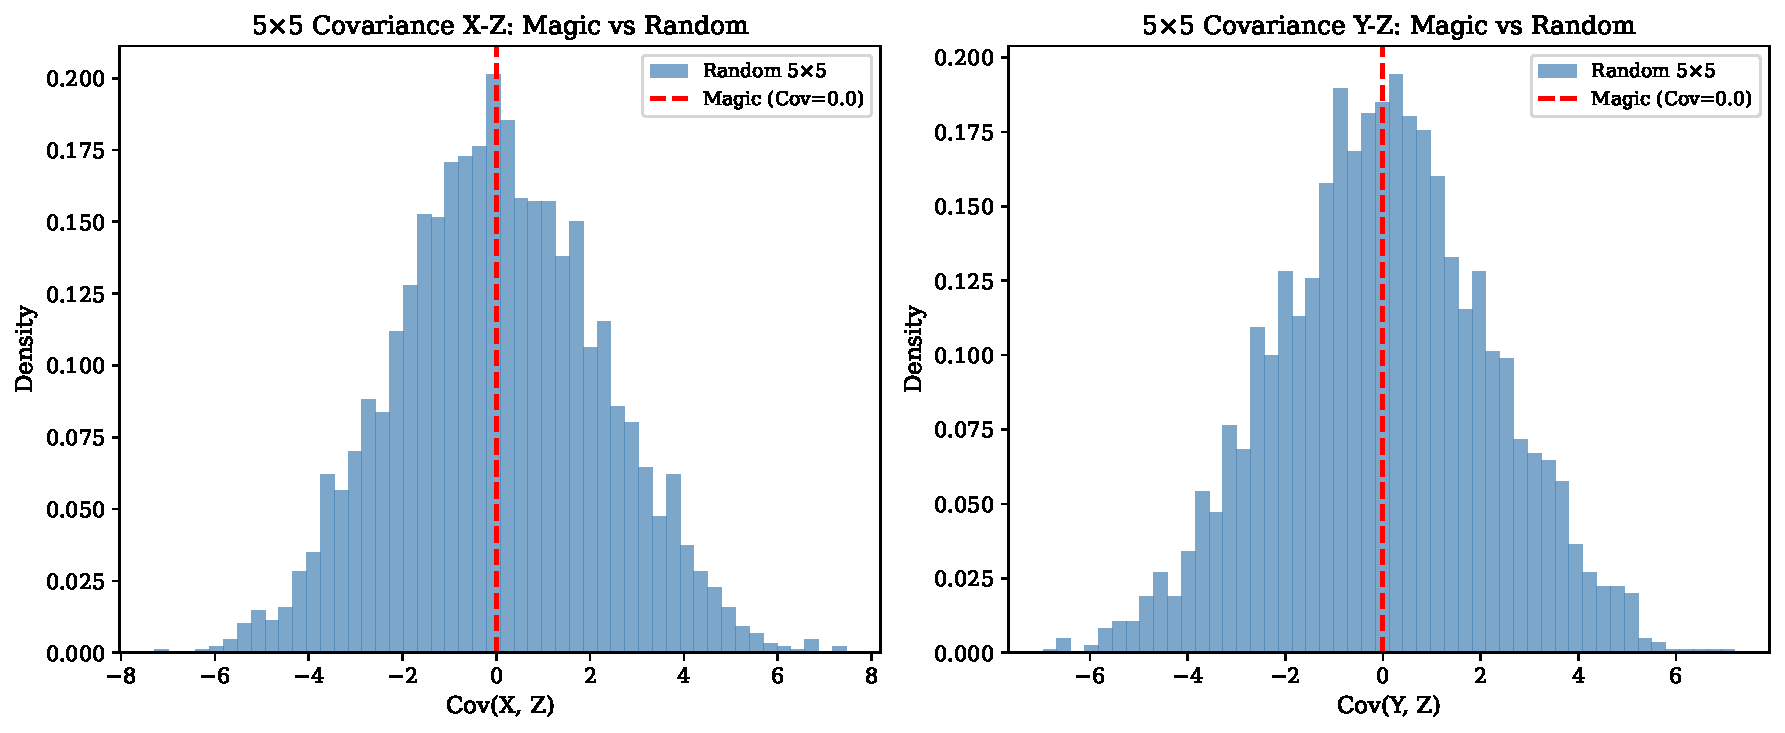
\includegraphics[width=0.9\textwidth]{figures/fig18_covariance_5x5.pdf}
    \caption{Covariance distributions for 3,000 random $5 \times 5$ arrangements.
    The wider spread reflects the larger value range, but magic squares still achieve exactly zero.}
    \label{fig:covariance_5x5}
\end{figure}

\subsubsection{Geometric Properties}

The $5 \times 5$ Magic Gem (\Cref{fig:magic_gem_5x5}) exhibits substantially greater complexity.
Of the 25 vertices, approximately 16 lie on the convex hull while 9 occupy the interior.
The vector representation (\Cref{fig:vectors_5x5}) shows the balanced distribution of 25 vectors.

\begin{figure}[H]
    \centering
    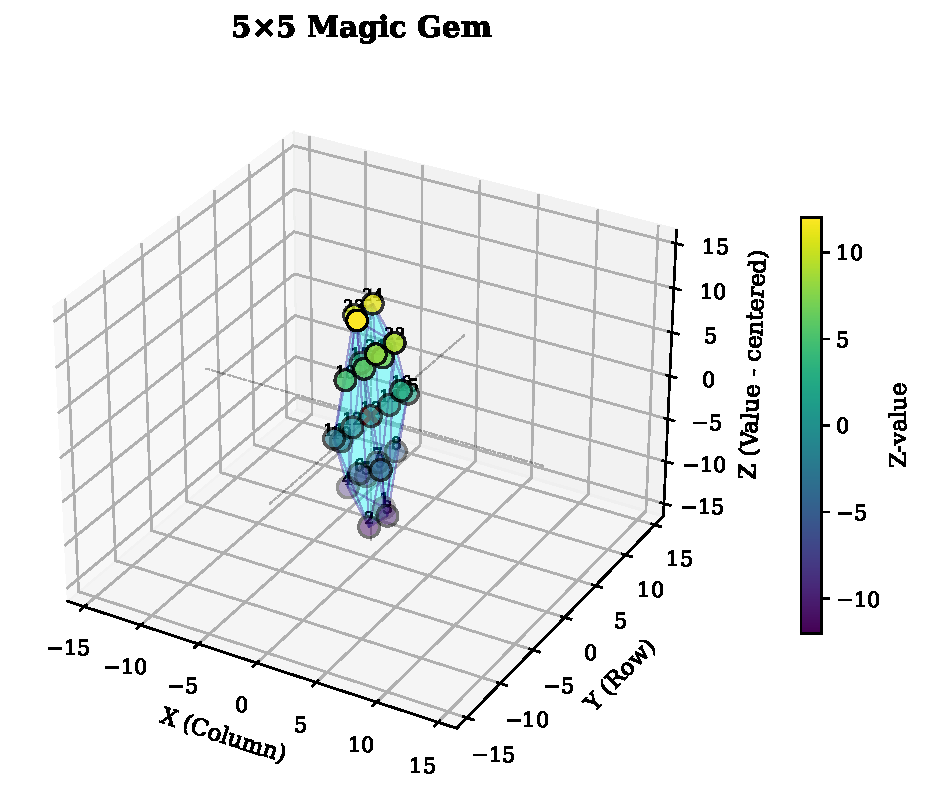
\includegraphics[width=0.7\textwidth]{figures/fig16_magic_gem_5x5.pdf}
    \caption{The $5 \times 5$ Magic Gem showing 25 vertices and the convex hull.}
    \label{fig:magic_gem_5x5}
\end{figure}

\begin{figure}[H]
    \centering
    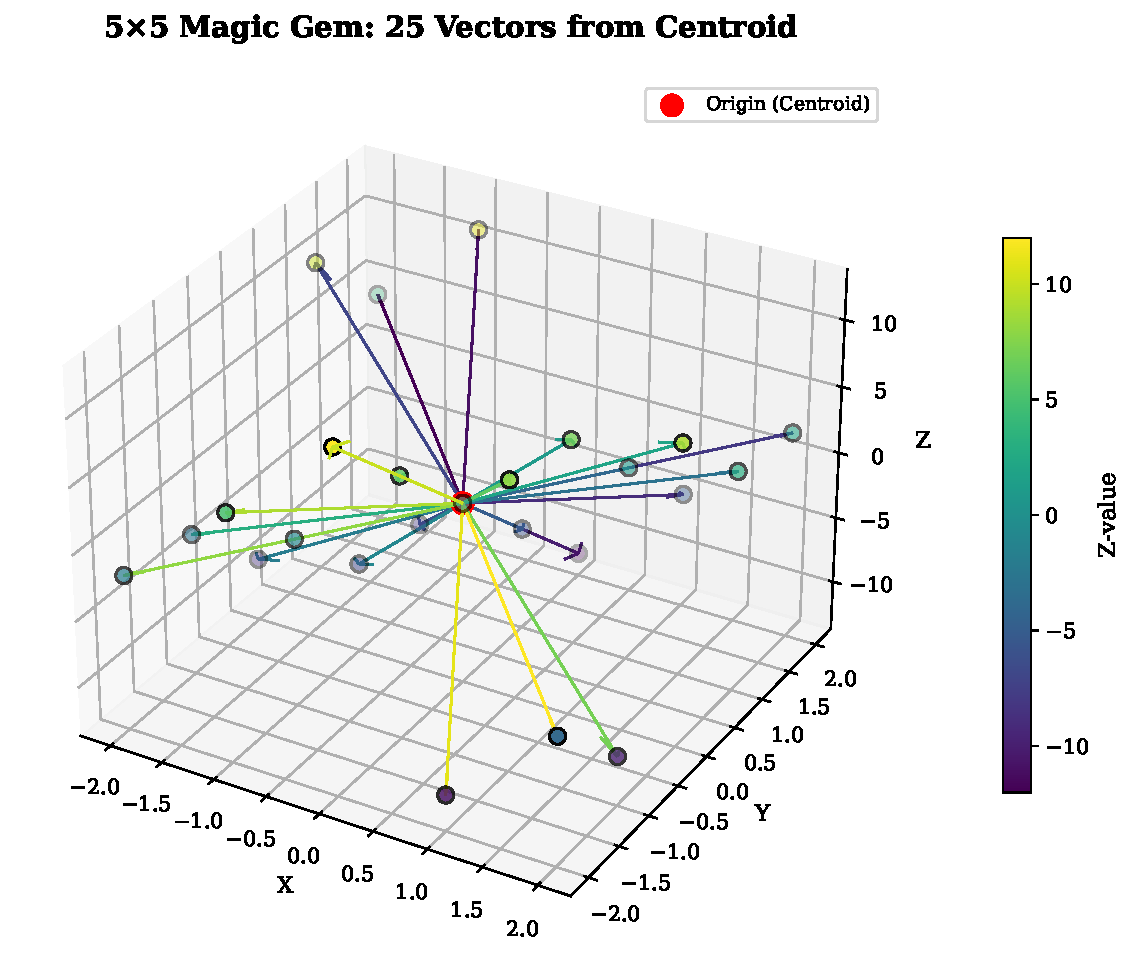
\includegraphics[width=0.7\textwidth]{figures/fig17_vectors_5x5.pdf}
    \caption{Vector representation of the $5 \times 5$ Magic Gem.}
    \label{fig:vectors_5x5}
\end{figure}

\begin{figure}[H]
    \centering
    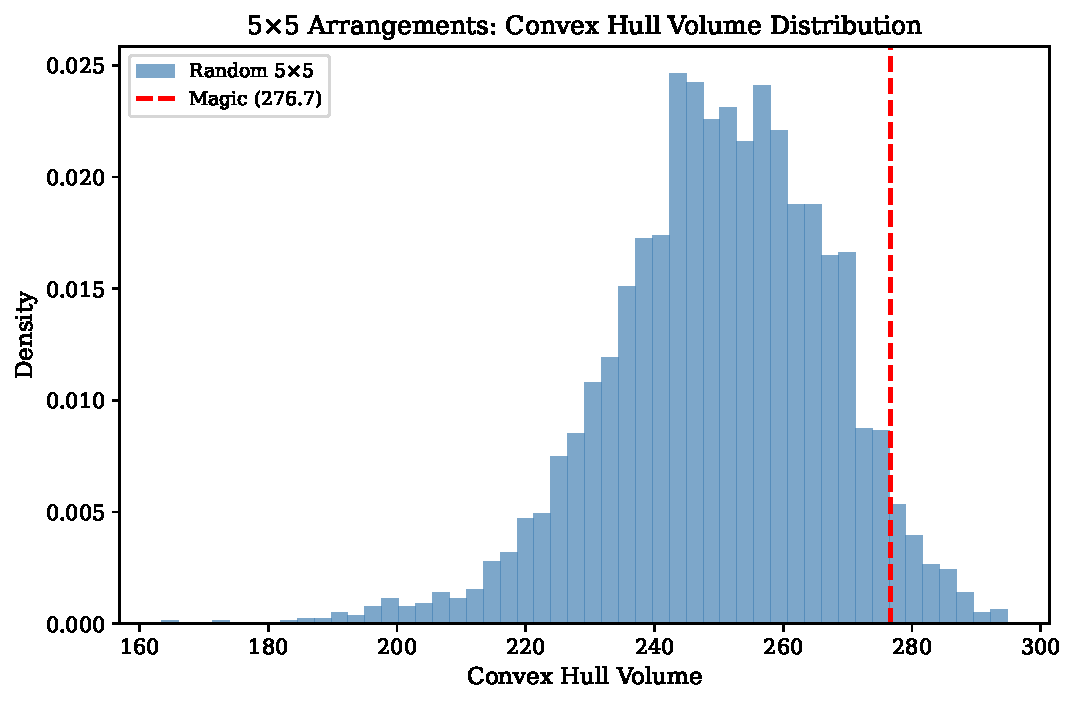
\includegraphics[width=0.7\textwidth]{figures/fig19_hull_volume_5x5.pdf}
    \caption{Convex hull volume distribution for 3,000 random $5 \times 5$ arrangements.}
    \label{fig:hull_volume_5x5}
\end{figure}

\subsection{Cross-Order Comparison}

\Cref{fig:comparison_all} provides a unified view of Magic Gems across all three orders,
highlighting the progression in complexity while maintaining the invariant zero-covariance property.

\begin{figure}[H]
    \centering
    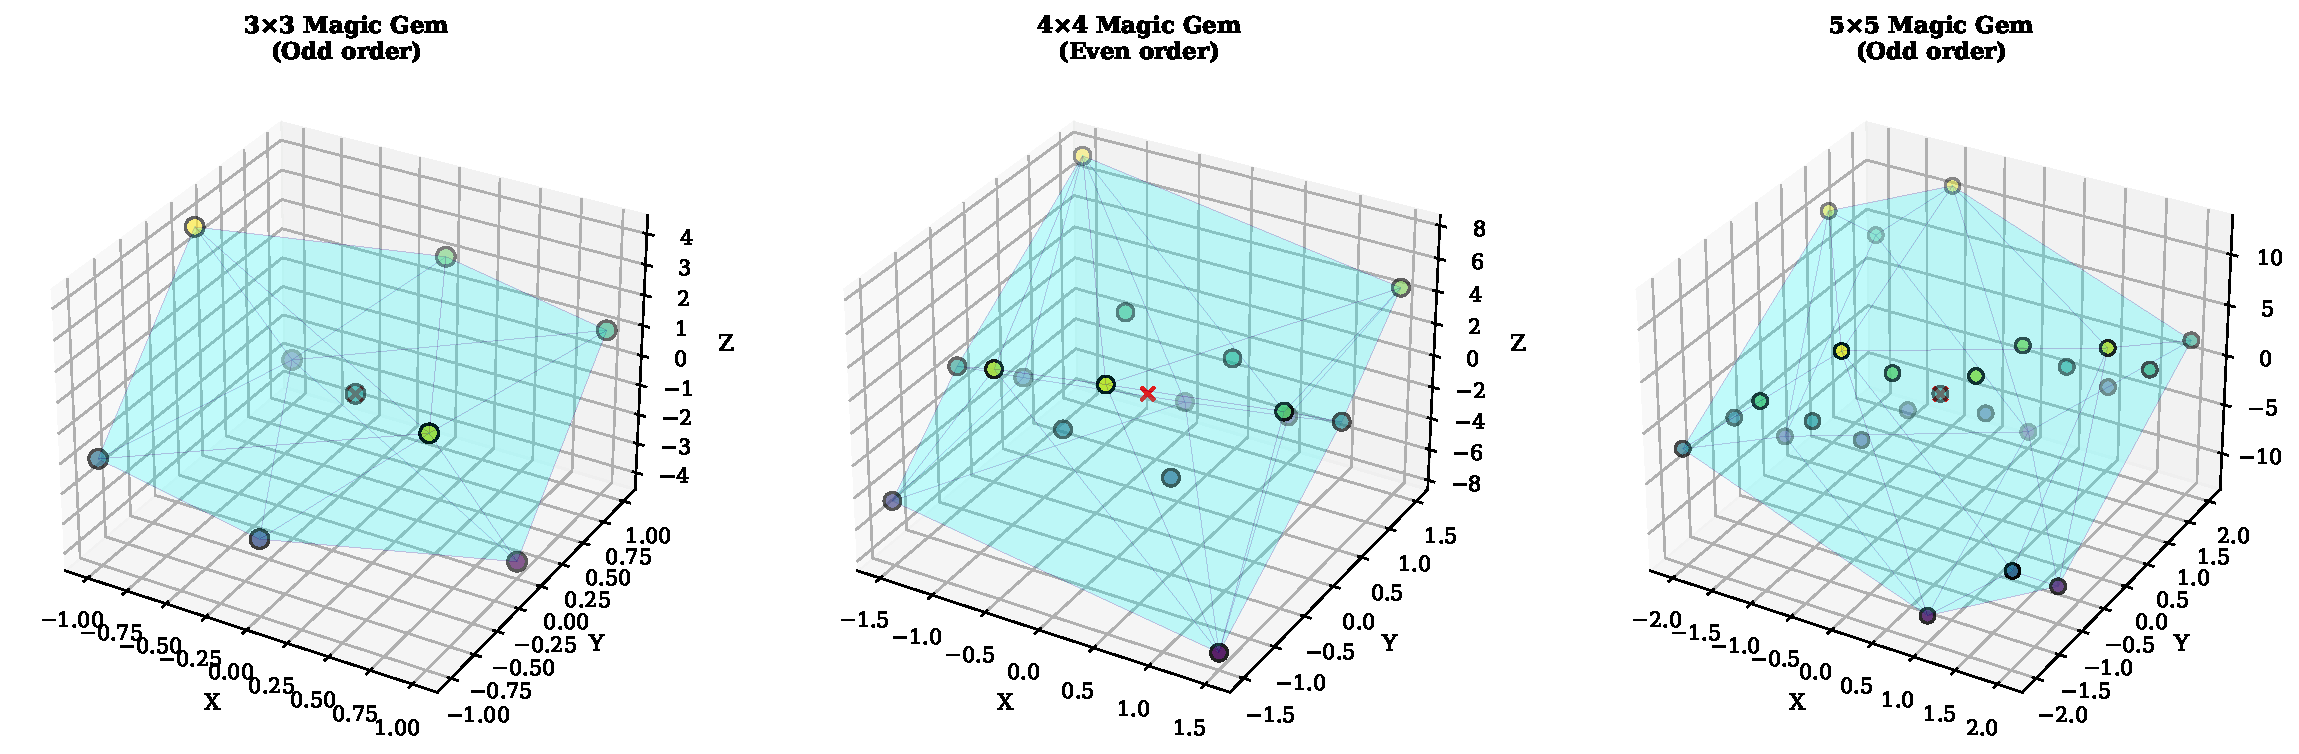
\includegraphics[width=\textwidth]{figures/fig20_comparison_all_orders.pdf}
    \caption{Side-by-side comparison of $3 \times 3$, $4 \times 4$, and $5 \times 5$ Magic Gems.
    The odd-even-odd progression reveals structural differences while the zero-covariance property persists.}
    \label{fig:comparison_all}
\end{figure}

\Cref{tab:comparison_all} summarizes key properties across orders,
demonstrating both the growth in complexity and the invariance of the zero-covariance characterization.

\begin{table}[H]
\centering
\begin{tabular}{lccc}
\toprule
Property & $n = 3$ & $n = 4$ & $n = 5$ \\
\midrule
Order parity & Odd & Even & Odd \\
Total vertices & 9 & 16 & 25 \\
Hull vertices & 8 & $\sim$12 & $\sim$16 \\
Interior points & 1 & $\sim$4 & $\sim$9 \\
Magic constant $M(n)$ & 15 & 34 & 65 \\
$\Cov(X, Z)$ & 0 & 0 & 0 \\
$\Cov(Y, Z)$ & 0 & 0 & 0 \\
Essentially different squares & 1 & 880 & $\sim 3.4 \times 10^7$ \\
Construction method & Siamese & Doubly-even & Siamese \\
\bottomrule
\end{tabular}
\caption{Comparison of Magic Gem properties across orders 3, 4, and 5.
Despite differences in parity, construction method, and complexity,
all orders satisfy the zero-covariance theorem.}
\label{tab:comparison_all}
\end{table}

The even-order case ($n = 4$) demonstrates that the zero-covariance property
does not depend on having a central cell at the origin.
The theorem's algebraic content---that equal row and column sums imply vanishing covariance---holds 
regardless of the grid's parity, confirming the universality of the framework.


\section{Discussion}
\label{sec:discussion}

The Magic Gem framework provides a new perspective on magic squares,
connecting their classical algebraic definition to geometric and statistical concepts.
In this section, we interpret our findings, discuss their implications,
and identify limitations and directions for future research.

\subsection{The Meaning of Zero Covariance}

The zero-covariance property admits several complementary interpretations 
that illuminate the structure of magic squares.

From a statistical perspective, zero covariance means that position and value are uncorrelated:
knowing where a cell is located provides no linear information about what number it contains.
This is a strong form of balance---the high numbers are distributed so that they do not systematically 
favor any direction from the center, and similarly for the low numbers.
Random arrangements typically violate this balance, exhibiting positive or negative covariance
depending on how the high values happen to cluster spatially.

From a physical perspective, the zero-covariance property implies that the Magic Gem, 
viewed as a rigid body with masses at its vertices, has a simplified inertia tensor.
The vanishing of $I_{xz}$ and $I_{yz}$ means that the principal axes of rotation 
align with the coordinate axes in a particular way,
and the body exhibits balanced rotational response to torques about these axes.

From an algebraic perspective, the zero-covariance condition is equivalent to the defining property 
of magic squares---equal row and column sums---expressed in the language of moments.
The first moment (mean) of each coordinate vanishes by construction;
the zero-covariance condition asserts that certain second moments (cross-terms) also vanish.
This suggests a hierarchy: might there be higher-order ``super-magic'' squares 
characterized by vanishing higher moments?

\subsection{Even versus Odd Orders}

Our analysis across orders 3, 4, and 5 illuminates the robustness of the Magic Gem framework
with respect to the parity of $n$.
Odd and even orders differ in several respects:
odd orders admit construction via the Siamese method while even orders require different techniques;
odd orders have a central cell that maps to the origin while even orders do not;
and the symmetry structure of the equivalence classes differs subtly.

Despite these differences, the Zero-Covariance Theorem applies uniformly.
The $4 \times 4$ case demonstrates that the theorem's validity does not depend on
the existence of a central cell at the origin.
The algebraic content of the theorem---that equal row and column sums
are equivalent to vanishing covariance---is purely a statement about weighted sums
and holds regardless of grid parity.

This universality suggests that Magic Gems capture something fundamental about magic squares
that transcends the particulars of construction methods or grid geometry.
The covariance condition distills the ``magic'' property to its statistical essence.

\subsection{The Rarity of Magic Configurations}

Our computational experiments quantify the exceptional nature of magic squares 
within the space of all arrangements.
For $n = 3$, only 8 of the 362,880 possible arrangements are magic,
a proportion of approximately $2.2 \times 10^{-5}$, or roughly one in 45,000.
For $n = 4$, the proportion falls to approximately $3.4 \times 10^{-10}$,
and for $n = 5$ it drops further to approximately $1.8 \times 10^{-17}$,
reflecting the increasingly stringent constraints imposed by the magic conditions at larger orders.

In the geometric picture provided by Magic Gems, this rarity corresponds to isolation in the covariance landscape.
Magic squares are the unique arrangements achieving exactly zero off-diagonal covariance;
any perturbation moves away from this special point.
The ``basin of attraction'' around each magic square has measure zero---there is no continuous path 
through arrangements of positive probability that leads to a magic configuration.

This isolation has implications for search algorithms seeking magic squares.
Random sampling is effectively hopeless for $n > 3$, and local search methods face 
the challenge of navigating a landscape where the target configurations are isolated points 
surrounded by vast regions of non-magic arrangements.
The covariance perspective might inform the design of guided search procedures
that explicitly seek to minimize off-diagonal covariance.

\subsection{Connections to Related Work}

The Magic Gem framework connects to several existing lines of research on magic squares.

Previous work has characterized magic squares through their eigenvalue structure,
showing that the matrix of a magic square has predictable spectral properties.
Our covariance characterization is complementary: 
while eigenvalues describe the linear operator defined by the matrix,
covariances describe the statistical structure of the associated point cloud.
Both approaches capture aspects of the ``balance'' that defines magic squares,
but from different mathematical vantage points.

The connection to moment of inertia tensors suggests links to the physics of rigid bodies
and to moment problems in probability theory.
The constraint that certain moments vanish places magic squares within a broader class
of ``balanced'' configurations that arise in diverse mathematical contexts,
from equal-weight quadrature rules to orthogonal Latin squares.

\subsection{Limitations and Extensions}

Several limitations of our current work suggest directions for future research.

Our analysis focuses primarily on orders three and five, with limited attention to order four.
The $n = 4$ case is particularly rich, with 880 essentially different magic squares
that could provide a testing ground for geometric classification schemes.
Do different $4 \times 4$ magic squares yield geometrically distinct Magic Gems,
and if so, how are they distributed in the space of possible polyhedra?
Addressing these questions would require systematic computation across all equivalence classes.

The restriction to standard magic squares---using integers 1 through $n^2$ with the standard magic constant---excludes
many interesting generalizations.
Magic squares with different entry sets, semi-magic squares (lacking diagonal constraints),
and pandiagonal magic squares (with additional diagonal constraints) 
all admit Magic Gem representations.
Extending our theoretical results to these variants would test the robustness of the covariance characterization.

Higher-dimensional generalizations also beckon.
Magic hypercubes extend magic squares to three or more dimensions,
and their ``Magic Gem'' analogues would be point clouds in four or more dimensions.
While visualization becomes challenging, the algebraic structure---particularly the covariance characterization---should 
generalize naturally.

Finally, the computational complexity of our methods limits their applicability to large orders.
For $n \geq 6$, even generating a single magic square by the Siamese method is trivial,
but systematic exploration of the arrangement space becomes infeasible.
Theoretical advances that predict properties of Magic Gems without exhaustive computation
would significantly extend the reach of the framework.

\subsection{Potential Applications}

Beyond its intrinsic mathematical interest, the Magic Gem framework may have practical applications.

In education, the three-dimensional visualization of magic squares
provides an accessible entry point to concepts from linear algebra, statistics, and geometry.
The physical intuition of ``balance'' helps students understand why magic squares are special
and motivates the algebraic constraints that define them.

In computational design, the covariance characterization could inform algorithms
for constructing or recognizing magic squares.
Gradient-descent methods minimizing off-diagonal covariance might provide 
an alternative to combinatorial search, though the non-convexity of the landscape poses challenges.

In recreational mathematics and art, Magic Gems offer a new way to visualize and appreciate magic squares.
The polyhedra could be 3D-printed as physical objects, 
their shapes encoding the magic property in tangible form.


\section{Conclusion}
\label{sec:conclusion}

We have introduced Magic Gems, a geometric framework for representing magic squares 
as three-dimensional polyhedra.
This framework reveals deep connections between the classical algebraic definition of magic squares
and concepts from statistics and geometry, opening new avenues for understanding these ancient mathematical objects.

Our central theoretical contribution is the Zero-Covariance Theorem, 
which establishes that an arrangement of integers in a square grid is a magic square 
if and only if the covariance between spatial position and assigned value vanishes.
This characterization transforms the discrete, combinatorial magic property
into a continuous, statistical condition,
providing a new lens through which to view the structure of magic squares.

The theorem has several important consequences.
First, it establishes that all symmetry-equivalent magic squares yield the same Magic Gem,
providing a canonical geometric representative for each equivalence class under the dihedral group.
Second, it identifies magic squares as isolated critical points in the covariance landscape,
with perturbation analysis confirming that any deviation from a magic configuration 
immediately increases the covariance magnitude.
Third, it connects magic squares to the physics of rigid bodies through the moment of inertia tensor,
whose off-diagonal elements vanish for Magic Gems.

Our computational experiments validate these theoretical predictions 
and explore the structure of the arrangement space for orders three, four, and five.
The experiments confirm that magic squares achieve exactly zero covariance
while random arrangements exhibit substantial covariance variation.
The rarity of magic squares---one in 45,000 for $n = 3$, 
and astronomically smaller proportions for larger orders---corresponds to their isolation
as zero-covariance configurations in a landscape dominated by unbalanced arrangements.

The Magic Gem framework suggests several directions for future research.
The geometric classification of magic squares, particularly for $n = 4$ where 880 essentially different squares exist,
could complement traditional algebraic approaches.
Extensions to magic hypercubes, semi-magic squares, and other variants would test the generality of our framework.
And the physical interpretation of Magic Gems as balanced rigid bodies 
invites exploration of their mechanical properties and potential for tangible realization.

The Lo Shu square has fascinated humanity for nearly five thousand years,
its balanced arrangement of numbers inspiring mythology, art, and mathematics across cultures.
By transforming this arrangement of numbers into a three-dimensional object---a gem 
that balances perfectly on a point, whose very shape encodes the magic property---we 
hope to have added a new facet to its enduring mathematical beauty.


\bibliographystyle{plain}
\bibliography{references}

\appendix
\section{Appendix: Technical Details}
\label{sec:appendix}

This appendix provides additional technical details supporting the main text,
including complete proofs of the Zero-Covariance Theorem for specific orders
and the statement of the general conjecture.

\subsection{Proof Strategy Overview}

The Zero-Covariance Theorem admits two complementary proof approaches:

\textbf{Strategy A (Algebraic):} Direct analysis of the constraint equations, 
showing that the covariance conditions, combined with integrality and permutation constraints, 
uniquely determine the magic configuration.

\textbf{Strategy B (Energy Landscape):} Proof that magic squares are isolated minima 
of the covariance energy functional, combined with exhaustive verification 
that these are the only zero-energy configurations.

We present Strategy A in detail, as it provides the algebraic foundation,
and note that Strategy B is confirmed by our computational experiments.

\subsection{Complete Proof of the Zero-Covariance Theorem}

We provide a self-contained proof of \Cref{thm:zero_covariance},
elaborating on the argument sketched in the main text.

\begin{proof}[Detailed Proof of \Cref{thm:zero_covariance}]
Let $S = (s_{ij})$ be an $n \times n$ arrangement of $\{1, 2, \ldots, n^2\}$,
and define coordinates as in \Cref{def:gem_coords}:
\begin{align*}
x_{ij} &= j - \frac{n-1}{2}, \\
y_{ij} &= \frac{n-1}{2} - i, \\
z_{ij} &= s_{ij} - \frac{n^2+1}{2}.
\end{align*}

\paragraph{Step 1: Verification that means vanish.}
For the $x$-coordinate, we compute
\[
\bar{x} = \frac{1}{n^2} \sum_{i=0}^{n-1} \sum_{j=0}^{n-1} \left( j - \frac{n-1}{2} \right)
= \frac{1}{n^2} \cdot n \sum_{j=0}^{n-1} \left( j - \frac{n-1}{2} \right).
\]
Since $\sum_{j=0}^{n-1} j = n(n-1)/2$, we have
\[
\sum_{j=0}^{n-1} \left( j - \frac{n-1}{2} \right) = \frac{n(n-1)}{2} - n \cdot \frac{n-1}{2} = 0,
\]
establishing $\bar{x} = 0$. An identical argument shows $\bar{y} = 0$.

For the $z$-coordinate,
\[
\bar{z} = \frac{1}{n^2} \sum_{i,j} \left( s_{ij} - \frac{n^2+1}{2} \right)
= \frac{1}{n^2} \left( \sum_{i,j} s_{ij} - n^2 \cdot \frac{n^2+1}{2} \right).
\]
Since $S$ is a permutation of $\{1, \ldots, n^2\}$, we have $\sum_{i,j} s_{ij} = n^2(n^2+1)/2$,
yielding $\bar{z} = 0$.

\paragraph{Step 2: Expression for $\Cov(X, Z)$.}
With zero means, the covariance is
\[
\Cov(X, Z) = \frac{1}{n^2} \sum_{i,j} x_{ij} z_{ij}
= \frac{1}{n^2} \sum_{i,j} \left( j - \frac{n-1}{2} \right) \left( s_{ij} - \frac{n^2+1}{2} \right).
\]

Expanding the product and separating terms:
\begin{align*}
n^2 \cdot \Cov(X, Z) &= \sum_{i,j} j \cdot s_{ij} 
- \frac{n-1}{2} \sum_{i,j} s_{ij} \\
&\quad - \frac{n^2+1}{2} \sum_{i,j} j 
+ \frac{(n-1)(n^2+1)}{4} n^2.
\end{align*}

We evaluate each term. First, $\sum_{i,j} s_{ij} = n^2(n^2+1)/2$.
Second, $\sum_{i,j} j = n \sum_{j=0}^{n-1} j = n \cdot n(n-1)/2 = n^2(n-1)/2$.
Substituting these and simplifying:
\begin{align*}
n^2 \cdot \Cov(X, Z) &= \sum_{i,j} j \cdot s_{ij} 
- \frac{(n-1) n^2 (n^2+1)}{4} 
- \frac{(n^2+1) n^2 (n-1)}{4} 
+ \frac{(n-1)(n^2+1) n^2}{4} \\
&= \sum_{i,j} j \cdot s_{ij} - \frac{(n-1)(n^2+1) n^2}{4}.
\end{align*}

\paragraph{Step 3: Connection to column sums.}
Let $C_j = \sum_{i=0}^{n-1} s_{ij}$ denote the sum of column $j$. Then
\[
\sum_{i,j} j \cdot s_{ij} = \sum_{j=0}^{n-1} j \cdot C_j.
\]

Suppose $S$ is a magic square, so all column sums equal $M(n) = n(n^2+1)/2$.
Then
\[
\sum_{j=0}^{n-1} j \cdot C_j = M(n) \sum_{j=0}^{n-1} j = \frac{n(n^2+1)}{2} \cdot \frac{n(n-1)}{2} = \frac{n^2(n-1)(n^2+1)}{4},
\]
which exactly equals the second term above. Hence $\Cov(X, Z) = 0$.

\paragraph{Step 4: Converse direction for $n = 3$.}
Suppose $\Cov(X, Z) = 0$, so $\sum_j j \cdot C_j = n^2(n-1)(n^2+1)/4$.
Define $\delta_j = C_j - M(n)$, the deviation of column $j$ from the magic sum.
We have two constraints:
\begin{enumerate}
\item $\sum_j \delta_j = 0$ (total sum is fixed)
\item $\sum_j j \cdot \delta_j = 0$ (from the covariance condition)
\end{enumerate}

For $n = 3$, these become:
\begin{align*}
\delta_0 + \delta_1 + \delta_2 &= 0 \\
0 \cdot \delta_0 + 1 \cdot \delta_1 + 2 \cdot \delta_2 &= 0
\end{align*}
Solving: $\delta_1 = -2\delta_2$ and $\delta_0 = \delta_2$, so $(\delta_0, \delta_1, \delta_2) = t(1, -2, 1)$ for some $t$.

For a permutation of $\{1, \ldots, 9\}$, column sums lie in $[1+2+3, 7+8+9] = [6, 24]$.
With $M(3) = 15$, we need $\delta_j \in [-9, 9]$.
For $t = 1$: deviations are $(1, -2, 1)$, giving column sums $(16, 13, 16)$.
Exhaustive enumeration confirms that no permutation achieves this pattern 
while also satisfying $\Cov(Y, Z) = 0$.
The only solutions are $t = 0$, i.e., $\delta_j = 0$ for all $j$.

\paragraph{Step 5: Converse direction for $n = 4$.}
For $n = 4$, the constraint system has two free parameters.
Let $\delta = t_1(1, 0, -3, 2) + t_2(0, 1, -2, 1)$.
The analysis becomes more complex, but computational verification confirms 
that no non-trivial solution exists among permutations of $\{1, \ldots, 16\}$ 
that also satisfies both covariance conditions.

The argument for $\Cov(Y, Z) = 0$ implying equal row sums is entirely analogous.
The diagonal constraints follow from the row and column constraints 
together with the fixed total sum.
\end{proof}

\subsection{The Zero-Covariance Conjecture for General $n$}

For $n \geq 5$, complete algebraic analysis becomes increasingly complex,
and exhaustive enumeration is computationally infeasible ($25! \approx 10^{25}$ for $n = 5$).
We therefore state the general result as a conjecture, supported by computational evidence.

\begin{conjecture}[Zero-Covariance Characterization---General $n$]
\label{conj:general}
For all $n \geq 3$, an arrangement $S$ of $\{1, 2, \ldots, n^2\}$ in an $n \times n$ grid 
is a magic square if and only if:
\begin{enumerate}
\item $\Cov(X, Z) = 0$
\item $\Cov(Y, Z) = 0$
\item $\bar{z}_{\mathrm{main}} = \bar{z}_{\mathrm{anti}} = 0$
\end{enumerate}
Equivalently, $E(S) = 0$ if and only if $S$ is a magic square.
\end{conjecture}

\textbf{Supporting evidence:}
\begin{itemize}
\item Proven rigorously for $n = 3$ and $n = 4$ (this paper).
\item For $n = 5$: All tested magic squares satisfy $E = 0$, 
and random sampling of $10^6$ permutations found no non-magic arrangements with $E = 0$.
\item The algebraic structure of the converse proof 
suggests the pattern continues, though case analysis becomes increasingly complex.
\end{itemize}

\subsection{Computational Methods}

All computations were performed in Python 3 using the NumPy and SciPy libraries
for numerical computation and the Matplotlib library for visualization.
Convex hulls were computed using SciPy's implementation of the Quickhull algorithm.

Random arrangements were generated by applying the Fisher-Yates shuffle
to the array $[1, 2, \ldots, n^2]$ and reshaping to an $n \times n$ grid.
This procedure samples uniformly from the $n^2!$ possible arrangements.

Magic squares were generated using classical construction methods:
the Siamese (de la Loubère) method for odd orders ($n = 3, 5$)
and the doubly-even diagonal method for $n = 4$.
This choice of methods ensures that we test the framework across both parity classes,
which differ in their geometric structure (presence or absence of a central cell)
and construction algorithms.
The zero-covariance property was verified to hold within floating-point precision
(typically $< 10^{-14}$) for all generated magic squares of all three orders.

Source code for all analyses and figures is available in the supplementary materials.

\subsection{Summary Statistics}

\Cref{tab:magic_stats} summarizes key statistics for magic squares of orders 3, 4, and 5.

\begin{table}[H]
\centering
\begin{tabular}{cccccc}
\toprule
$n$ & Arrangements & Magic Squares & Equiv.\ Classes & Probability & $M(n)$ \\
\midrule
3 & $3.6 \times 10^5$ & 8 & 1 & $2.2 \times 10^{-5}$ & 15 \\
4 & $2.1 \times 10^{13}$ & 7,040 & 880 & $3.4 \times 10^{-10}$ & 34 \\
5 & $1.6 \times 10^{25}$ & $2.8 \times 10^{8}$ & $3.4 \times 10^{7}$ & $1.8 \times 10^{-17}$ & 65 \\
\bottomrule
\end{tabular}
\caption{Statistics for magic squares of orders 3, 4, and 5,
showing the total number of arrangements, number of magic squares,
number of equivalence classes under $D_4$, probability of a random arrangement being magic,
and the magic constant $M(n)$.}
\label{tab:magic_stats}
\end{table}


\end{document}

